%\documentclass[handout]{beamer}
\documentclass{beamer}
 
\usetheme[numbering = fraction, progressbar = none, background = light, sectionpage = progressbar]{metropolis}
\usepackage{amsmath}
\usepackage{tabu}
\usepackage{graphicx}
\usepackage{hyperref}
\usepackage{xcolor}
\usepackage{tikz}
\usepackage{setspace}
\usetikzlibrary{shapes,backgrounds,trees}

\title{Econ 103 -- Statistics for Economists}
\subtitle{Chapter 6 and 7: Confidence Intervals}
\author{Mallick Hossain}
\date{}
\institute{University of Pennsylvania}
\begin{document} 

%%%%%%%%%%%%%%%%%%%%%%%%%%%%%%%%%%%%%%%%
\begin{frame}
	\titlepage 
\end{frame} 

\section{3 Students}
%%%%%%%%%%%%%%%%%%%%%%%%%%%%%%%%%%%%%%%%
\begin{frame}
\frametitle{Lost Larry}
\centering

\includegraphics[scale=0.7]{./images/whatsthepoint1.jpeg}
\end{frame}

%%%%%%%%%%%%%%%%%%%%%%%%%%%%%%%%%%%%%%%%
\begin{frame}
\frametitle{Smart Spider-Man}
\centering

\includegraphics[scale=0.5]{./images/whatsthepoint2.jpg}
\end{frame}

%%%%%%%%%%%%%%%%%%%%%%%%%%%%%%%%%%%%%%%%
\begin{frame}
\frametitle{Synthesizing Squirrel}
\centering

\includegraphics[scale=0.7]{./images/iUnderstand.jpg}
\end{frame}

%%%%%%%%%%%%%%%%%%%%%%%%%%%%%%%%%%%%%%%%
\begin{frame}
\frametitle{What's the Point?}
The goal is to get you closer to the squirrel (or at least Spider-Man)
\end{frame}

\section{Recap and Motivation}
%%%%%%%%%%%%%%%%%%%%%%%%%%%%%%%%%%%%%%%%
\begin{frame}
\frametitle{What We've Done So Far (Theory Side)}

\begin{itemize}[<+-|alert@+>]
\item We spent the past few weeks covering discrete and continuous random variables
	\begin{itemize}
		\item You should be very comfortable with each random variable and their associated properties (see random variable handout for a nice (not necessarily exhaustive) summary)
	\end{itemize}
	\item We dug into the normal distribution and all of its nice properties
	\begin{itemize}
		\item The more intuitive the normal RV feels, the easier the rest of the semester will be
	\end{itemize}
	\item Briefly introduced chi-squared, t-, and F-distributions
	\begin{itemize}
		\item You'll see why they are so important today! The wait is over!
	\end{itemize}
\end{itemize}
\end{frame}

%%%%%%%%%%%%%%%%%%%%%%%%%%%%%%%%%%%%%%%%
\begin{frame}
\frametitle{What We've Done So Far (Practical Side)}

\begin{itemize}
\item Random Sampling: $X_1, \hdots, X_n \sim \mbox{ iid}$ 
\item Use estimator $\widehat{\theta}$ to learn about population parameter $\theta_0$ 
\item Estimator $\widehat{\theta}$ is a random variable: 
	\begin{itemize}
		\item Distribution of $\widehat{\theta}$ is called \emph{sampling distribution}
		\item Bias of an estimator 
		\item Variance of an estimator 
		\item Mean-squared Error (MSE) of an estimator 
		\item Consistency of an Estimator
	\end{itemize}
\end{itemize}
\end{frame}

%%%%%%%%%%%%%%%%%%%%%%%%%%%%%%%%%%%%%%%%
\begin{frame}
\frametitle{The Road Ahead}

\begin{block}{Confidence Intervals}
What values of $\theta_0$ are consistent with the data we observed?
\end{block}

\begin{block}{Hypothesis Testing}
I think that $\theta_0 = 0$. Should I change my mind based on the data?
\end{block}

\end{frame}

%%%%%%%%%%%%%%%%%%%%%%%%%%%%%%%%%%%%%%%%
\begin{frame}
\frametitle{Motivation}
\begin{itemize}[<+-|alert@+>]
	\item Do we expect point estimates to be exactly right?
	\begin{itemize}
		\item No! As we saw last lecture, our estimate is basically a draw from the distribution of a random variable
	\end{itemize}
	\item If we predicted that the S\&P 500 would close at \$2150.00 on Monday and it closed at \$2150.88, my point estimate was wrong. Does that mean it's worthless though?
	\begin{itemize}
		\item No! It was ``close'' which can be very informative!
		\item Confidence intervals are instrumental in giving us a better idea of what counts as ``close.''
	\end{itemize}
\end{itemize}

\end{frame}

\section{Example}
%%%%%%%%%%%%%%%%%%%%%%%%%%%%%%%%%%%%%%%%
\begin{frame}
\frametitle{(Above?) Average Joe }

Joe is 73 inches tall. Based on a sample of US males aged 20 and over, the Centers for Disease Control (CDC) reported a mean height of about 69 inches in a recent report.

\alert{Clearly Joe is taller than the average American male!}\\
Do you agree or disagree?
\begin{enumerate}[(a)]
	\item Agree
	\item Disagree
	\item Not Sure
\end{enumerate}
\end{frame}

%%%%%%%%%%%%%%%%%%%%%%%%%%%%%%%%%%%%%%%%
\begin{frame}
\frametitle{Remember: The Sample Mean is Random!}

\alert{Just because the sample mean is 69 inches it doesn't follow that the population mean is 69 inches!}

\begin{block}{What Else Should We Consider?}
	\begin{itemize}\pause
		\item How big was the sample? \pause
			\begin{itemize}
				\item If the sample was very small there's a higher chance that it won't be representative of the population as a whole \pause
				\item Why? The variance of the sample mean is \emph{decreasing with sample size} so bigger samples are less noisy. \pause
			\end{itemize}
		\item How much variability is there in height in the population?	\pause
			\begin{itemize}
				\item If everyone is very similar in height, any sample we take will be representative of the population. \pause
				\item Remember: the variance of the sample mean is \emph{increasing} with the population standard deviation. 
			\end{itemize}
	\end{itemize}
\end{block}

\end{frame}

%%%%%%%%%%%%%%%%%%%%%%%%%%%%%%%%%%%%%%%%
\begin{frame}
\frametitle{Am I Taller Than The Average American Male?}
	
	\begin{table}[h]
	\caption{Height in inches for Males aged 20 and over (approximate)}
		\begin{tabular}{|lr|}
		\hline
			Sample Mean & 69 inches\\
			Sample Std.\ Dev.\ & 6 inches\\
			Sample Size & 5647 \\
			\hline
			Joe's Height & 73 inches\\
			\hline
		\end{tabular}
	\end{table}

\vspace{2em}
\alert{We'll return to this example later.}

\end{frame}

\section{Theoretical Example}
%%%%%%%%%%%%%%%%%%%%%%%%%%%%%%%%%%%%%%%%
\begin{frame}
\frametitle{For Now -- Single Population, Normally Distributed}
\Large
$$\boxed{X_1, X_2, \hdots, X_n\sim \mbox{iid } N(\mu,\sigma^2)}$$


\vspace{4em}
\normalsize
\alert{Later we'll look at more than one population and talk about what happens if Normality doesn't hold.}
\end{frame}

%%%%%%%%%%%%%%%%%%%%%%%%%%%%%%%%%%%%%%%%
\begin{frame}
Suppose $X_1, X_2, \hdots, X_n \sim \mbox{iid } N(\mu,\sigma^2)$. What is the sampling distribution of $\sqrt{n}(\bar{X}_n - \mu)/\sigma$?


\begin{enumerate}[(a)]
\item $N(\mu, \sigma^2)$
\item $N(0,1)$
\item $N(0,\sigma)$
\item $N(\mu, 1)$
\item Not enough information to determine.
\end{enumerate}

\end{frame}

%%%%%%%%%%%%%%%%%%%%%%%%%%%%%%%%%%%%%%%%
\begin{frame}
\frametitle{Z-score!}
Suppose $X_1, X_2, \hdots, X_n \sim \mbox{iid } N(\mu,\sigma^2)$. From above,
	\begin{eqnarray*}
			E[\bar{X}_n] &=& \mu\\
			Var(\bar{X}_n) &=&  \sigma^2/n\\ 
			&\Rightarrow& SD(\bar{X}_n) =\sigma/\sqrt{n}
	\end{eqnarray*} 
Thus,
	$$\sqrt{n}(\bar{X}_n - \mu)/\sigma =  \frac{\bar{X}_n - \mu}{\sigma/\sqrt{n}} =  \frac{\bar{X}_n - E[\bar{X}_n]}{SD(\bar{X}_n)}  \sim N(0,1)$$
Remember that we call the standard deviation of a sampling distribution the \alert{standard error}, written $SE$, so $$\frac{\bar{X}_n - \mu}{SE(\bar{X}_n)} \sim N(0,1)$$
\end{frame}

%%%%%%%%%%%%%%%%%%%%%%%%%%%%%%%%%%%%%%%%
\begin{frame}
\frametitle{Standard Error vs Standard Deviation}
\begin{itemize}
	\item \textbf{Standard Deviation}
	\begin{itemize}
		\item The square root of the variance
		\item Measures the deviation from the mean
	\end{itemize}
	\item \textbf{Standard Error}
	\begin{itemize}
		\item A specific kind of standard deviation
		\item This is the standard deviation of the estimator
		\item For example, if we are estimating the population mean, the standard error tells us how far our estimate is from the actual population mean.
	\end{itemize}
\end{itemize}
\end{frame}

%%%%%%%%%%%%%%%%%%%%%%%%%%%%%%%%%%%%%%%%
\begin{frame}
Suppose $X_1, X_2, \hdots, X_n \sim \mbox{iid } N(\mu,\sigma^2)$. What is the approximate value of the following?
$$P\left(-2 \leq \frac{\bar{X}_n - \mu}{SE(\bar{X}_n)} \leq 2 \right)\pause \alert{\approx 0.95}$$

\end{frame}

%%%%%%%%%%%%%%%%%%%%%%%%%%%%%%%%%%%%%%%%
\begin{frame}
\frametitle{What happens if I rearrange?}
	\begin{eqnarray*}
		P\left(-2 \leq \frac{\bar{X}_n - \mu}{SE(\bar{X}_n)} \leq 2 \right) &=& 0.95\\ \\ \pause
			P\left(-2\cdot SE\leq \bar{X}_n - \mu \leq 2 \cdot SE\right) &=& 0.95\\ \\ \pause
			P\left(-2\cdot SE - \bar{X}_n \leq - \mu \leq 2 \cdot SE - \bar{X}_n \right) &=& 0.95\\ \\ \pause
			\alert{P\left( \bar{X}_n - 2\cdot SE \leq \mu \leq \bar{X}_n + 2\cdot SE \right)}&\alert{=}& \alert{0.95}
	\end{eqnarray*}

\end{frame}

\section{Confidence Intervals}
%%%%%%%%%%%%%%%%%%%%%%%%%%%%%%%%%%%%%%%%
\begin{frame}
\frametitle{Confidence Intervals}

\begin{block}{Confidence Interval (CI)}
A confidence interval is a range $(A,B)$ constructed from the \alert{sample data} that has a specified probability of containing a \alert{population parameter}:
	$$P(A \leq \theta_0 \leq B) = 1-\alpha$$
\end{block} 

\pause

\begin{block}{Confidence Level}
The \alert{specified probability}, typically denoted $1-\alpha$, is called the confidence level. For example, if $\alpha = 0.05$ then the confidence level is 0.95 or 95\%.
\end{block}
\end{frame}

%%%%%%%%%%%%%%%%%%%%%%%%%%%%%%%%%%%%%%%%
\begin{frame}
\frametitle{Confidence Interval for Mean of Normal Population}
\framesubtitle{Population Variance Known}


\begin{block}{Confidence Interval for Mean of Normal Population}
	The interval \alert{$\boxed{\bar{X}_n \pm 2 \sigma/\sqrt{n}}$} has approximately 95\% probability of containing the population mean $\mu$, provided that:
		$$\boxed{X_1, X_2, \hdots, X_n\sim \mbox{iid } N(\mu,\sigma^2)}$$
\end{block}

\pause

\begin{alertblock}{But What Does This Mean?}
\end{alertblock}

\end{frame}

%%%%%%%%%%%%%%%%%%%%%%%%%%%%%%%%%%%%%%%%
\begin{frame}
\frametitle{Which quantities are random?}
Suppose $X_1, X_2, \hdots, X_n\sim \mbox{iid } N(\mu,\sigma^2)$.
Which quantities are random variables?
	\begin{enumerate}[(a)]
\item $\mu$ only
\item $\sigma$ and $\mu$
\item $\sigma$ only
\item $\sigma, \mu$ and $\bar{X}_n$
\item \only<2->{\alert}{$\bar{X}_n$ only}
\end{enumerate}

\vspace{1em}
\pause
\alert{What does this mean for our confidence intervals?}

\end{frame}

%%%%%%%%%%%%%%%%%%%%%%%%%%%%%%%%%%%%%%%%
\begin{frame}
\frametitle{Confidence Interval is a Random Variable!}
\begin{enumerate}
	\item $X_1, \hdots, X_n$ are RVs $\Rightarrow \bar{X}_n$ is a RV (repeated sampling) \pause
	\item $\mu$, $\sigma$ and $n$ are constants \pause
	\item Confidence Interval $\bar{X_n}\pm 2 \sigma/\sqrt{n}$ is also a RV!
\end{enumerate}

\end{frame}

%%%%%%%%%%%%%%%%%%%%%%%%%%%%%%%%%%%%%%%
\begin{frame}
\frametitle{Meaning of Confidence Interval}
\begin{block}{Meaning of Confidence Interval}
If we sampled many times we'd get many different sample means, each leading to a \alert{different} confidence interval. Approximately 95\% of these intervals will contain $\mu$.
\end{block}
 

\begin{block}{Rough Intuition}
What values of $\mu$ are consistent with the data?
\end{block}

\end{frame}

%%%%%%%%%%%%%%%%%%%%%%%%%%%%%%%%%%%%%%%
\begin{frame}
\frametitle{CI for Population Mean: Repeated Sampling}

\begin{center}
\setlength{\unitlength}{1cm}
\begin{picture}(5,7)
\put(-0.5,6){\framebox(6,1){$X_1, X_2, \hdots, X_n \sim \mbox{iid } N(\mu, \sigma^2)$}}

\pause

\put(0.5,6){\vector(-1,-1){1.5}}
\put(-2.3,3.7){\framebox(2.5,0.65){Sample 1}}

\pause

\put(-1,3.5){\vector(0,-1){0.75}}
\put(-1.25,2.1){\framebox(0.5,0.5){\small $\bar{x}_1$}}

\pause

\put(-1,2){\vector(0,-1){0.5}}
\put(-1.7,1){{\small $\bar{x}_1 \pm 2\sigma/\sqrt{n}$}}

\pause

\put(2,6){\vector(0,-1){1.5}}
\put(0.7,3.7){\framebox(2.5,0.65){Sample 2}}

\pause

\put(2,3.5){\vector(0,-1){0.75}}
\put(1.75,2.1){\framebox(0.5,0.5){\small $\bar{x}_2$}}

\pause

\put(2,2){\vector(0,-1){0.5}}
\put(1.35,1){{\small $\bar{x}_2 \pm 2\sigma/\sqrt{n}$}}

\pause

\put(3.8,4){\makebox{...}}
\put(3.8,2.3){\makebox{...}}

\pause

\put(4.5,6){\vector(1,-1){1.5}}
\put(4.8,3.7){\framebox(2.5,0.65){Sample M}}

\pause

\put(6,3.5){\vector(0,-1){0.75}}
\put(5.75,2.1){\framebox(0.5,0.5){\small $\bar{x}_M$}}

\pause

\put(6,2){\vector(0,-1){0.5}}
\put(5.35,1){{\small $\bar{x}_M \pm 2\sigma/\sqrt{n}$}}

\pause

\put(-1,0.2){\makebox{\small Repeat $M$ times $\rightarrow$  get $M$ different intervals}}

\pause

\put(-1,-0.3){\makebox{\small \alert{Large M $\Rightarrow$ Approx.\ 95\% of these Intervals Contain $\mu$}}}

\end{picture}
\end{center}


\end{frame}

%%%%%%%%%%%%%%%%%%%%%%%%%%%%%%%%%%%%%%%%
\begin{frame}
\frametitle{Simulation Example: $X_1, \hdots, X_5 \sim \mbox{iid } N(0,1)$, $M = 20$}

\begin{figure}
\centering
\includegraphics[scale = 0.5]{./images/CIs1}
\caption{Twenty confidence intervals of the form $\bar{X}_n \pm 2 \sigma/\sqrt{n}$ where $n=5$, $\sigma^2 = 1$ and the true population mean is $0$.}
\end{figure}

\end{frame}

%%%%%%%%%%%%%%%%%%%%%%%%%%%%%%%%%%%%%%%%
\begin{frame}
\frametitle{Meaning of Confidence Interval for $\theta_0$}
	$$\boxed{P(A\leq \theta_0 \leq B) = 1-\alpha}$$
Each time we sample we'll get a different confidence interval, corresponding to different realizations of the random variables $A$ and $B$. If we sample many times, approximately $100\times(1-\alpha)$\% of these intervals will contain the population parameter $\theta_0$.

\end{frame}

%%%%%%%%%%%%%%%%%%%%%%%%%%%%%%%%%%%%%%%%
\begin{frame}
\frametitle{True or False? }
Suppose 
	$$\boxed{X_1, X_2, \hdots, X_n\sim \mbox{iid } N(\mu,\sigma^2)}$$
Then the population mean $\mu$ has approximately a 95\% chance of falling in the interval $\bar{X}_n \pm 2 \sigma/\sqrt{n}$.

\vspace{1em}

\begin{enumerate}[(a)]
\item True
\item False
\end{enumerate}


\pause
\vspace{1em}
\alert{\huge FALSE! -- $\mu$  is a constant!}


\end{frame}

%%%%%%%%%%%%%%%%%%%%%%%%%%%%%%%%%%%%%%%%
\begin{frame}
\frametitle{Confidence Intervals: Some Terminology}
\begin{block}{Margin of Error}
When a CI takes the form $\widehat{\theta}\pm ME$, $ME$ is the Margin of Error. 
\end{block}
\pause
\begin{block}{Lower and Upper Confidence Limits}
The lower endpoint of a CI is the \alert{lower confidence limit (LCL)}, while the upper endpoint is the \alert{upper confidence limit (UCL)}.
\end{block}
\pause
\begin{block}{Width of a Confidence Interval}
The distance $\alert{|\mbox{UCL} - \mbox{LCL}|}$ is called the \alert{width} of a CI. This means exactly what it says. 
\end{block}

\end{frame}

\section{Margin of Error}
%%%%%%%%%%%%%%%%%%%%%%%%%%%%%%%%%%%%%%%%
\begin{frame}
\frametitle{What is the Margin of Error}
In the preceding example of a  95\% confidence interval for the mean of a normal population when the population variance is known, which of these is the margin of error?
	\begin{enumerate}[(a)]
		\item $\sigma/\sqrt{n}$
		\item $\bar{X}_n$
		\item $\sigma$
		\item $2\sigma/\sqrt{n}$
		\item $1/\sqrt{n}$
	\end{enumerate}
\pause
\vspace{1em}
\alert{\large $2\sigma/\sqrt{n}$, since the CI is $\bar{X}_n \pm 2\sigma/\sqrt{n}$}
\end{frame}

%%%%%%%%%%%%%%%%%%%%%%%%%%%%%%%%%%%%%%%%
\begin{frame}
\frametitle{What is the Width?}
In the preceding example of a  95\% confidence interval for the mean of a normal population when the population variance is known, which of these is the width of the interval?
	\begin{enumerate}[(a)]
		\item $\sigma/\sqrt{n}$
		\item $2\sigma/\sqrt{n}$
		\item $3\sigma/\sqrt{n}$
		\item $4\sigma/\sqrt{n}$
		\item $5\sigma/\sqrt{n}$
	\end{enumerate}
\pause
\vspace{1em}
\alert{\large $4\sigma/\sqrt{n}$, since the CI is $\bar{X}_n \pm 2\sigma/\sqrt{n}$}
\end{frame}
%%%%%%%%%%%%%%%%%%%%%%%%%%%%%%%%%%%%%%%%
\begin{frame}
\frametitle{Example: Calculate the Margin of Error }
\begin{center}\fbox{\begin{minipage}{0.75\textwidth}
$X_1, \hdots, X_{100} \sim \mbox{iid } N(\mu, 1)$ but we don't know $\mu$. Want to create a 95\% confidence interval for $\mu$.
\end{minipage}}
\end{center}
What is the margin of error?
\pause

\vspace{2em}

The confidence interval is $\bar{X}_n \pm 2\sigma/\sqrt{n}$ so 
	$$\alert{ME = 2\sigma/\sqrt{n} = 2 \cdot 1/\sqrt{100} = 2/10 = 0.2}$$

\end{frame}

%%%%%%%%%%%%%%%%%%%%%%%%%%%%%%%%%%%%%%%%
\begin{frame}
\frametitle{Example: Calculate the Lower Confidence Limit }


\begin{center}\fbox{\begin{minipage}{0.75\textwidth}
$X_1, \hdots, X_{100} \sim N(\mu, 1)$ but we don't know $\mu$. Want to create a 95\% confidence interval for $\mu$.
\end{minipage}}
\end{center}

We found that $ME=0.2$. The sample mean $\bar{x} = 4.9$. What is the lower confidence limit?
\pause

\vspace{2em}

	$$\alert{\mbox{LCL} = \bar{x} - ME= 4.9 - 0.2 = 4.7}$$

\end{frame}

%%%%%%%%%%%%%%%%%%%%%%%%%%%%%%%%%%%%%%%%
\begin{frame}
  \frametitle{Example: Similarly for the Upper Confidence Limit\dots}


\begin{center}\fbox{\begin{minipage}{0.75\textwidth}
$X_1, \hdots, X_{100} \sim N(\mu, 1)$ but we don't know $\mu$. Want to create a 95\% confidence interval for $\mu$.
\end{minipage}}
\end{center}

We found that $ME=0.2$. The sample mean $\bar{x} = 4.9$. What is the upper confidence limit?
\pause

\vspace{2em}

	$$\alert{\mbox{UCL} = \bar{x} + ME= 4.9 + 0.2 = 5.1}$$

\end{frame}

%%%%%%%%%%%%%%%%%%%%%%%%%%%%%%%%%%%%%%%%
\begin{frame}
\frametitle{Example: 95\% CI for Normal Mean, Popn.\ Var.\ Known}

\begin{center}\fbox{\begin{minipage}{0.75\textwidth}
$X_1, \hdots, X_{100} \sim N(\mu, 1)$ but we don't know $\mu$.
\end{minipage}}
\end{center}

	$$\alert{\mbox{95\% CI for } \mu = [4.7, 5.1]}$$

What values of $\mu$ are plausible?

\pause
\vspace{1em}

\alert{The data actually came from a $N(5,1)$ Distribution.}

\end{frame}

%%%%%%%%%%%%%%%%%%%%%%%%%%%%%%%%%%%%%%%%
\begin{frame}
\frametitle{Want to be more certain? Use higher confidence level.}
What value of $c$ should we use to get a 100$\times(1-\alpha)$\% CI for $\mu$?
	\begin{eqnarray*}
		P\left(-c \leq \frac{\bar{X}_n-\mu}{\sigma/\sqrt{n}} \leq c \right) &=& 1-\alpha \\ \\ \pause
		P\left(\bar{X}_n - c \sigma/\sqrt{n} \leq \mu\leq \bar{X}_n + c \sigma/\sqrt{n} \right) &=& 1-\alpha 
	\end{eqnarray*}
 \pause

\alert{Take $c =$ \texttt{qnorm}$(1-\alpha/2)$} \pause
	$$\bar{X}_n \pm \texttt{qnorm}(1-\alpha/2) \times \sigma/\sqrt{n}$$
\end{frame}

%%%%%%%%%%%%%%%%%%%%%%%%%%%%%%%%%%%%%%%%
\begin{frame}
\begin{figure}
\centering
\includegraphics[scale = 0.6]{./images/normal_tails}
\end{figure}
\end{frame}
%%%%%%%%%%%%%%%%%%%%%%%%%%%%%%%%%%%%%%%%
\begin{frame}
\frametitle{Confidence Interval for a Normal Mean, $\sigma$ Known}
\Large
$$\boxed{\bar{X}_n \pm \texttt{qnorm}(1-\alpha/2) \times \sigma/\sqrt{n}}$$
\end{frame}

%%%%%%%%%%%%%%%%%%%%%%%%%%%%%%%%%%%%%%%%
\begin{frame}
\frametitle{What Affects the Margin of Error?}

	$$\boxed{\bar{X}_n \pm \texttt{qnorm}(1-\alpha/2) \times \sigma/\sqrt{n}}$$


	
\begin{block}{Sample Size $n$}
ME decreases with $n$: bigger sample $\implies$ tighter interval
\end{block}


\begin{block}{Population Std.\ Dev.\ $\sigma$}
ME increases with $\sigma$: more variable population $\implies$ wider interval
\end{block}



\begin{block}{Confidence Level $1-\alpha$}
ME increases with $1-\alpha$: higher conf.\ level $\implies$ wider interval

\pause

\vspace{1em}
\centering
	\begin{tabular}{r|lll}
	\hline
	Conf.\ Level & 90\% & 95\% & 99\% \\
	$\alpha$ & 0.1 & 0.05 & 0.01\\
	\texttt{qnorm}$(1-\alpha/2)$&1.64 & 1.96 & 2.56\\
	\hline
	\end{tabular}
\end{block}	
\end{frame}

%%%%%%%%%%%%%%%%%%%%%%%%%%%%%%%%%%%%%%%%
\begin{frame}
\frametitle{But What if $\sigma$ is Unknown?}
	\begin{itemize}
		\item What we've done so far assumed that $\sigma$ was known. 
		\item In real applications this is typically not the case. 
		\only<2->{\item So what do we do now?}
	\end{itemize}
\end{frame}

%%%%%%%%%%%%%%%%%%%%%%%%%%%%%%%%%%%%%%%%
\begin{frame}
\frametitle{The Suspense!}
\centering
	
\includegraphics[scale=0.3]{./images/cliffhanger.jpg}
\end{frame}

%%%%%%%%%%%%%%%%%%%%%%%%%%%%%%%%%%%%%%%%
\begin{frame}
\frametitle{We Don't know $\sigma$. What to use instead?}
$$\boxed{\bar{X}_n \pm \texttt{qnorm}(1-\alpha/2) \times \sigma/\sqrt{n}}$$

\begin{block}{What about Sample Standard Deviation $S$?}
	$$P\left(-2 \leq \frac{\bar{X}_n-\mu}{S/\sqrt{n}} \leq 2 \right) = 0.95 \mbox{ ???}$$
\end{block}

\begin{block}{Not Quite!}
Although $(\bar{X}_n-\mu)/(\sigma/\sqrt{n})\sim N(0,1)$, $S \neq \sigma$. In fact, $S$ is an \alert{estimator} of $\sigma$ so it is a \alert{random variable!}
\end{block}
\end{frame}

%%%%%%%%%%%%%%%%%%%%%%%%%%%%%%%%%%%%%%%%
\begin{frame}
\frametitle{What is the sampling distribution?}
Suppose $X_1, \hdots, X_n \sim N(\mu,\sigma^2)$
 $$\boxed{\frac{\bar{X}_n-\mu}{S/\sqrt{n}}  \sim \mbox{ ???}}$$

 \begin{block}{First Step}
What is the sampling distribution of $S$?
\end{block}
\end{frame}

%%%%%%%%%%%%%%%%%%%%%%%%%%%%%%%%%%%%%%%%
\begin{frame}
\frametitle{What is the Distribution? }
Suppose $X_1, \hdots, X_n \sim N(\mu,\sigma^2)$. What is the distribution of this sum?
	$$\sum_{i=1}^n \left(\frac{X_i - \mu}{\sigma}\right)^2$$
	
	\begin{enumerate}[(a)]
\item $\chi^2(n)$
\item $N(\mu, \sigma^2)$
\item $N(0,1)$
\item $N(\mu, \sigma^2/n)$
\item $\chi^2(1)$
\end{enumerate}
\end{frame}

%%%%%%%%%%%%%%%%%%%%%%%%%%%%%%%%%%%%%%%%
\begin{frame}
\frametitle{Towards the Sampling Dist.\ of $S$}
If $X_1, \hdots, X_n \sim N(\mu,\sigma^2)$, then 
$$\sum_{i=1}^n \left(\frac{X_i - \mu}{\sigma}\right)^2 \sim \chi^2(n)$$

Now:
$$\sum_{i=1}^n \left(\frac{X_i - \mu}{\sigma}\right)^2   = \pause \left(\frac{n-1}{\sigma^2}\right) \left[\frac{1}{n-1}\sum_{i=1}^n \left(X_i - \mu\right)^2\right] \pause \sim \chi^2(n) $$
\alert{Anything look familiar?}
\end{frame}

%%%%%%%%%%%%%%%%%%%%%%%%%%%%%%%%%%%%%%%%
\begin{frame}
\frametitle{Sampling Distribution of Sample Variance}
Suppose $X_1, \hdots, X_n \sim N(\mu,\sigma^2)$. Then whereas
$$\left(\frac{n-1}{\sigma^2}\right) \left[\frac{1}{n-1}\sum_{i=1}^n \left(X_i - \mu\right)^2\right] \sim \chi^2(n)$$
\pause
Replacing $\mu$ with $\bar{X}$ ``loses'' a degree of freedom
	$$\left(\frac{n-1}{\sigma^2}\right) \left[\frac{1}{n-1}\sum_{i=1}^n \left(X_i - \bar{X}\right)^2\right] =\pause\alert{ \left(\frac{n-1}{\sigma^2}\right)S^2} \pause \alert{\sim \chi^2(n-1)}$$


\alert{Ultimately, we will use this fact to work out the sampling distribution of $\sqrt{n}(\bar{X}_n-\mu)/S$, but for now let's take a detour...}
\end{frame}

\section{Detour}
%%%%%%%%%%%%%%%%%%%%%%%%%%%%%%%%%%%%%%%%
\begin{frame}
\frametitle{95\% CI for Variance of Normal Population}
We know that:
	$$\left( \frac{n-1}{\sigma^2}\right)S^2\sim \chi^2(n-1)$$
	\pause
	\vspace{2em}
	
First Step: find $a,b$ such that 
	$$P\left[ a\leq   \left( \frac{n-1}{\sigma^2}\right)S^2 \leq b \right] = 0.95$$
	\pause
\alert{Although there are many choices for $a,b$ that would work, a sensible idea is to put 2.5\% in each tail...}
\end{frame}

%%%%%%%%%%%%%%%%%%%%%%%%%%%%%%%%%%%%%%%%
\begin{frame}
\begin{figure}
\centering
\includegraphics[scale = 0.65]{./images/chisq_tails}
\end{figure}
\end{frame}

%%%%%%%%%%%%%%%%%%%%%%%%%%%%%%%%%%%%%%%%
\begin{frame}
\frametitle{What R command should I use to calculate $a$? }
$$P\left[ a\leq   \left( \frac{n-1}{\sigma^2}\right)S^2 \leq b \right] = 0.95$$
	\begin{enumerate}[(a)]
		\item \texttt{qchisq}$( 0.95, \texttt{df = } n-1)$
		\item \texttt{qchisq}$( 0.025, \texttt{df = }  n)$
		\item \texttt{qchisq}$(0.975, \texttt{df = }  n-1)$
		\item \texttt{qchisq}$( 0.025, \texttt{df = }  n-1)$
		\item \texttt{qchisq}$(0.975, \texttt{df = }  n)$
	\end{enumerate}
\end{frame}

%%%%%%%%%%%%%%%%%%%%%%%%%%%%%%%%%%%%%%%%
\begin{frame}
\frametitle{What R command should I use to calculate $b$? }
$$P\left[ a\leq   \left( \frac{n-1}{\sigma^2}\right)S^2 \leq b \right] = 0.95$$
	\begin{enumerate}[(a)]
		\item \texttt{qchisq}$( 0.95, \texttt{df = } n-1)$
		\item \texttt{qchisq}$( 0.025, \texttt{df = }  n)$
		\item \texttt{qchisq}$(0.975, \texttt{df = }  n-1)$
		\item \texttt{qchisq}$( 0.025, \texttt{df = }  n-1)$
		\item \texttt{qchisq}$(0.975, \texttt{df = }  n)$
	\end{enumerate}
\end{frame}

%%%%%%%%%%%%%%%%%%%%%%%%%%%%%%%%%%%%%%%%
\begin{frame}
\begin{figure}
\centering
\includegraphics[scale = 0.55]{./images/chisq_tails}
\end{figure}

a = \texttt{qchisq(0.025, df = n - 1)} \\

b = \texttt{qchisq(0.975, df = n - 1)} 
\end{frame}

%%%%%%%%%%%%%%%%%%%%%%%%%%%%%%%%%%%%%%%%
\begin{frame}
\frametitle{Step 2: After Finding $a,b$ Rearrange}
 	\begin{eqnarray*}
 		P\left[ a\leq   \left( \frac{n-1}{\sigma^2}\right)S^2 \leq b \right] &=& 0.95 \\ \\ \pause
 		P\left[ \frac{a}{(n-1)S^2}\leq  \frac{1}{\sigma^2} \leq \frac{b}{(n-1)S^2} \right] &=& 0.95 \\ \\ \pause
 				P\left[ \frac{(n-1)S^2}{b}\leq  \sigma^2 \leq \frac{(n-1)S^2}{a} \right] &=& 0.95
 	\end{eqnarray*}	
 	\pause
\alert{This CI is \emph{not} symmetric: it \emph{doesn't} take the form $\widehat{\theta} \pm ME$!}
\end{frame}

%%%%%%%%%%%%%%%%%%%%%%%%%%%%%%%%%%%%%%%%
\begin{frame}
\frametitle{Example: 95\% Confidence Interval for Normal Variance}
$X_1, \hdots, X_{100} \sim N(\mu,\sigma^2)$. Here $n-1 = 99$, hence \pause
	\begin{eqnarray*}
		a = \texttt{qchisq(0.025, df = 99)} &\approx& 73\\ \pause
		b = \texttt{qchisq(0.975, df = 99)} &\approx& 128 \pause
	\end{eqnarray*}	
From the sample data, $s^2 = 4.3$
	\begin{eqnarray*}
		LCL &=& (n-1)s^2/b = \pause 99 \times 4.3/128 \pause \approx 3.3\\ \pause
		UCL &=& (n-1)s^2/a = \pause 99 \times 4.3/73 \pause \approx  5.8
	\end{eqnarray*}
	\pause
	\alert{95\% CI for $\sigma^2$ is $[3.3, 5.8]$. What values are plausible?}\\
	\pause
	The actual population variance in this case was 4
\end{frame}

%%%%%%%%%%%%%%%%%%%%%%%%%%%%%%%%%%%%%%%%
\begin{frame}
\frametitle{Arbitrary Confidence Level: $(1-\alpha)$}

\begin{figure}
\centering
\includegraphics[scale = 0.5]{./images/chisq_tails}
\end{figure}

a = \texttt{qchisq($\alpha/2$, df = n - 1)} \\

b = \texttt{qchisq($1-\alpha/2$, df = n - 1)} 
\end{frame}

%%%%%%%%%%%%%%%%%%%%%%%%%%%%%%%%%%%%%%%%
\begin{frame}
\frametitle{CI for Normal Variance}
a = \texttt{qchisq($\alpha/2$, df = n - 1)} \\
b = \texttt{qchisq($1-\alpha/2$, df = n - 1)} 
\vspace{1em}
 	\begin{eqnarray*}
 		P\left[ a\leq   \left( \frac{n-1}{\sigma^2}\right)S^2 \leq b \right] &=& 1-\alpha \\ \\
 		P\left[ \frac{a}{(n-1)S^2}\leq  \frac{1}{\sigma^2} \leq \frac{b}{(n-1)S^2} \right] &=& 1-\alpha \\ \\ 
 				P\left[ \frac{(n-1)S^2}{b}\leq  \sigma^2 \leq \frac{(n-1)S^2}{a} \right] &=& 1-\alpha
 	\end{eqnarray*}	
\end{frame}

%%%%%%%%%%%%%%%%%%%%%%%%%%%%%%%%%%%%%%%%
\begin{frame}
\frametitle{CI for Normal Variance}
Suppose $X_1, \hdots, X_n \sim \mbox{iid } N(\mu,\sigma^2)$ and let:
	\begin{eqnarray*}
		a &=& \texttt{qchisq($\alpha/2$, df = n - 1)} \\
		b &=& \texttt{qchisq($1-\alpha/2$, df = n - 1)} 
	\end{eqnarray*}
Then,
	$$\left[ \frac{(n-1)S^2}{b}, \frac{(n-1)S^2}{a} \right]$$
is a $100\times(1-\alpha)\%$ confidence interval for $\sigma^2$.
\end{frame}

%%%%%%%%%%%%%%%%%%%%%%%%%%%%%%%%%%%%%%%%
\begin{frame}
\frametitle{End of Detour}
We want to know the Sampling Distribution of $\sqrt{n}(\bar{X}_n - \mu)/S$ and we just saw that:
$$\boxed{\left( \frac{n-1}{\sigma^2}\right)S^2\sim \chi^2(n-1)}$$
\begin{alertblock}{How can we use this fact to help us?}
\end{alertblock}
\end{frame}

\section{Back on Track}
%%%%%%%%%%%%%%%%%%%%%%%%%%%%%%%%%%%%%%%%
\begin{frame}
\frametitle{What is the Sampling Distribution of $\sqrt{n}(\bar{X}_n-\mu)/S$?}
This slide is just algebra:
\begin{eqnarray*}
	\frac{\bar{X}_n - \mu}{S/\sqrt{n}} &=&\pause \frac{\bar{X}_n - \mu}{S/\sqrt{n}} \cdot \left(\frac{\sigma/\sqrt{n}}{\sigma/\sqrt{n}} \right) = \pause \left(\frac{\bar{X}_n - \mu}{\alert{\sigma/\sqrt{n}}} \right)\left(\frac{\sigma/\sqrt{n}}{\alert{S/\sqrt{n}}} \right)\\ \\
	&=& \pause\left(\frac{\bar{X}_n - \mu}{\sigma/\sqrt{n}} \right)\left(\frac{\sigma}{S} \right) = \pause  \left(\frac{\bar{X}_n - \mu}{\sigma/\sqrt{n}} \right)\left(\sqrt{\frac{n-1}{n-1}}\cdot\sqrt{\frac{\sigma^2}{S^2}} \right) \\ \\
	&=& \pause \left(\frac{\bar{X}_n - \mu}{\sigma/\sqrt{n}} \right)\left(\sqrt{\frac{(n-1)\sigma^2}{(n-1)S^2}} \right) \\ \\
	&=& \pause \frac{\displaystyle \left(\frac{\bar{X}_n - \mu}{\sigma/\sqrt{n}}\right)}{\sqrt{\left[\frac{(n-1)S^2}{\sigma^2}\right]/(n-1)}} 
\end{eqnarray*}
\end{frame}

%%%%%%%%%%%%%%%%%%%%%%%%%%%%%%%%%%%%%%%%
\begin{frame}[t]
\frametitle{Distribution of $\sqrt{n}(\bar{X}_n - \mu)/\sigma$ }
    
    Suppose $X_1, \hdots, X_n \sim \mbox{ iid } N(\mu, \sigma^2)$ and $\bar{X}_n$ is ths sample mean. Then the sampling distribution of \alert{$\sqrt{n}(\bar{X}_n - \mu)/\sigma$} is

    \begin{enumerate}[(a)]
    	\item $t(n)$
    	\item $t(n-1)$
    	\item $\chi^2(n)$
    	\item $\chi^2(n-1)$
    	\item $N(\mu, \sigma^2)$
    	\item $N(0,1)$
    	\item $N(\mu, \sigma^2/n)$
    	\item $F(n, n-1)$
    \end{enumerate}


\end{frame}

%%%%%%%%%%%%%%%%%%%%%%%%%%%%%%%%%%%%%%%%
\begin{frame}[c]
\frametitle{Distribution of $(n-1)S^2/\sigma^2$ }
    
    Suppose $X_1, \hdots, X_n \sim \mbox{ iid } N(\mu, \sigma^2)$ and $S^2$ is the sample variance. Then the sampling distribution of \alert{$(n-1)S^2/\sigma^2$} is

    \begin{enumerate}[(a)]
    	\item $t(n)$
    	\item $t(n-1)$
    	\item $\chi^2(n)$
    	\item $\chi^2(n-1)$
    	\item $N(\mu, \sigma^2)$
    	\item $N(0,1)$
    	\item $N(\mu, \sigma^2/n)$
    	\item $F(n, n-1)$
    \end{enumerate}


\end{frame}

%%%%%%%%%%%%%%%%%%%%%%%%%%%%%%%%%%%%%%%%
\begin{frame}[c]\frametitle{What is the Sampling Distribution? }
    
Suppose $Z\sim N(0,1)$ independent of $Y \sim \chi^2(n-1)$. Then the sampling distribution of \alert{$Z/\sqrt{Y/(n-1)}$} is

    \begin{enumerate}[(a)]
    	\item $t(n)$
    	\item $t(n-1)$
    	\item $\chi^2(n)$
    	\item $\chi^2(n-1)$
    	\item $N(\mu, \sigma^2)$
    	\item $N(0,1)$
    	\item $N(\mu, \sigma^2/n)$
    	\item $F(n, n-1)$
    \end{enumerate}



\end{frame}

%%%%%%%%%%%%%%%%%%%%%%%%%%%%%%%%%%%%%%%%
\begin{frame}
\frametitle{What is the Sampling Distribution of $\sqrt{n}(\bar{X}_n-\mu)/S$?}
From three slides back:
\begin{eqnarray*}
	\frac{\bar{X}_n - \mu}{S/\sqrt{n}} &=& \frac{\displaystyle \left(\frac{\bar{X}_n - \mu}{\sigma/\sqrt{n}}\right)}{\sqrt{\left[\frac{(n-1)S^2}{\sigma^2}\right]/(n-1)}} \\ \\ 
		&=&\pause \frac{N(0,1)}{\sqrt{\displaystyle\frac{\chi^2(n-1)}{n-1}}}\\ \\ 
		&\sim& \pause t(n-1)
\end{eqnarray*}
\pause
\alert{Strictly speaking, need to show that numerator and denominator are independent, but you can take my word for it!}
\end{frame}

%%%%%%%%%%%%%%%%%%%%%%%%%%%%%%%%%%%%%%%%
\begin{frame}
\frametitle{Punchline: Sampling Distribution of $\sqrt{n}(\bar{X}_n-\mu)/S$}
If $X_1, \hdots, X_n \sim \mbox{iid } N(\mu,\sigma^2)$, then
	$$\alert{\boxed{\frac{\bar{X}_n - \mu}{S/\sqrt{n}} \sim t(n-1)}}$$
\end{frame}

%%%%%%%%%%%%%%%%%%%%%%%%%%%%%%%%%%%%%%%%
\begin{frame}
\frametitle{Who was ``Student?''}
\begin{columns}

\column{0.3\textwidth}
\begin{figure}
\fbox{\includegraphics[scale = 0.05]{./images/gosset}}
\vspace{0.75em}

\includegraphics[scale = 0.17]{./images/guinness}
\end{figure}


\column{0.7\textwidth}
\footnotesize
\begin{quote}
``Student'' is the pseudonym used in 19 of 21 published articles by William Sealy
Gosset, who was a chemist, brewer, inventor, and self-trained statistician, agronomer, and designer of experiments ... [Gosset] worked his entire adult life ... as an experimental brewer for one employer: Arthur Guinness, Son \& Company, Ltd., Dublin, St.\ James’s Gate. Gosset was a master brewer and rose in fact to the top of the top of the brewing industry: Head Brewer of Guinness. \href{http://pubs.aeaweb.org/doi/pdfplus/10.1257/jep.22.4.199}{\color{blue}{Source}}
\end{quote}

\end{columns}

\end{frame}

%%%%%%%%%%%%%%%%%%%%%%%%%%%%%%%%%%%%%%%%
\begin{frame}
\frametitle{Three Key Sampling Distributions}
Suppose that $X_1, \hdots, X_n \sim \mbox{iid } N(\mu,\sigma^2)$. Then:

	\begin{eqnarray*}
		\left(\frac{n-1}{\sigma^2}\right) S^2&\sim&\chi^2(n-1)\\ \\
		\frac{\bar{X}_n-\mu}{\sigma/\sqrt{n}}&\sim& N(0,1)\\ \\
		\frac{\bar{X}_n-\mu}{S/\sqrt{n}}&\sim&t(n-1)
	\end{eqnarray*}
\end{frame}

%%%%%%%%%%%%%%%%%%%%%%%%%%%%%%%%%%%%%%%%
\begin{frame}
\frametitle{CI for Mean of Normal Distribution, Popn.\ Var.\ Unknown}
Same argument as we used when the variance was known, except with $t(n-1)$ rather than standard normal distribution:
	\begin{eqnarray*}
		P\left(-c \leq \frac{\bar{X}_n-\mu}{S/\sqrt{n}} \leq c \right) &=& 1-\alpha \\ \\ 
		P\left(\bar{X}_n - c \frac{S}{\sqrt{n}} \leq \mu\leq \bar{X}_n +c \frac{S}{\sqrt{n}} \right) &=& 1-\alpha 
	\end{eqnarray*}

\alert{$c =$ \texttt{qt}$(1-\alpha/2, \texttt{df} = n-1)$} 
	$$\boxed{\bar{X}_n \pm \texttt{qt}(1-\alpha/2, \texttt{df} = n-1)\;  \frac{S}{\sqrt{n}}}$$
\end{frame}

%%%%%%%%%%%%%%%%%%%%%%%%%%%%%%%%%%%%%%%%
\begin{frame}
\frametitle{Comparison of CIs for Mean of Normal Distribution}
\framesubtitle{$100\times(1-\alpha)\%$ Confidence Level}
$$\boxed{X_1, \hdots, X_n \sim \mbox{iid } N(\mu, \sigma^2)}$$


\begin{block}{Known Population Std.\ Dev.\ ($\sigma$)}
	$$\bar{X}_n \pm \; \texttt{qnorm}(1-\alpha/2) \; \frac{\sigma}{\sqrt{n}}$$
\end{block}


\begin{block}{Unknown Population Std.\ Dev.\ ($\sigma$)}
$$\bar{X}_n \pm \; \texttt{qt}(1-\alpha/2, \texttt{df} = n-1) \; \frac{S}{\sqrt{n}}$$
\end{block}
\end{frame}

%%%%%%%%%%%%%%%%%%%%%%%%%%%%%%%%%%%%%%%%
\begin{frame}
\frametitle{Standard Error vs.\ Estimator of Standard Error}
\begin{block}{Standard Error}
Recall that the standard deviation of  the sampling distribution of an estimator is called the \emph{\alert{standard error} (SE)} of that estimator.
\end{block}
\begin{block}{Example: Standard Error of the Mean}
$SE(\bar{X}_n) = \sqrt{Var\left(\bar{X_n}\right)} = \sigma/\sqrt{n}$
\end{block}



\begin{alertblock}{Estimator of Standard Error of the Mean} Whereas $\sigma/\sqrt{n}$ \alert{\emph{is}} the standard error of the mean, $S/\sqrt{n}$ is an \alert{\emph{estimator}} of this quantity: $\widehat{SE}(\bar{X_n}) = S/\sqrt{n}$
\end{alertblock}
\end{frame}

%%%%%%%%%%%%%%%%%%%%%%%%%%%%%%%%%%%%%%%%
\begin{frame}
\frametitle{Writing the CIs in terms of Actual and Estimated SE}
\framesubtitle{$100\times(1-\alpha)\%$ Confidence Level}
$$\boxed{X_1, \hdots, X_n \sim \mbox{iid } N(\mu, \sigma^2)}$$

\begin{block}{Known Population Std.\ Dev.\ ($\sigma$)}
	$$\bar{X}_n \pm \; \texttt{qnorm}(1-\alpha/2) \; \alert{SE(\bar{X}_n)}$$
\end{block}

\begin{block}{Unknown Population Std.\ Dev.\ ($\sigma$)}
$$\bar{X}_n \pm \; \texttt{qt}(1-\alpha/2, \texttt{df} = n-1) \; \alert{\widehat{SE}(\bar{X}_n)}$$
\end{block}
\end{frame}

%%%%%%%%%%%%%%%%%%%%%%%%%%%%%%%%%%%%%%%%
\begin{frame}
\frametitle{Comparison of Normal and $t$ CIs}
\begin{table}
\caption{Values of \texttt{qt}$(1-\alpha/2, \texttt{df}=n-1)$ for various choices of $n$ and $\alpha$. }
\begin{tabular}{r|rrrrr|r}
\hline
$n$& 1& 5& 10& 30& 100 & $\infty$\\
\hline
$\alpha = 0.10$&  6.31& 2.02 & 1.81 & 1.70  & 1.66 &1.64\\
$\alpha = 0.05$ & 12.71& 2.57 & 2.23 & 2.04  & 1.98 &1.96\\
$\alpha = 0.01$ & 63.66& 4.03 & 3.17 & 2.75  & 2.63 &2.58\\
\hline
\end{tabular}
\end{table}
\alert{Recall that as $n\rightarrow \infty$, $t(n-1) \rightarrow N(0,1)$}
\vspace{1em}


In a sense, using the $t$-distribution involves making a ``small-sample correction.'' In other words, it is only when $n$ is fairly small that this makes a practical difference for our confidence intervals.
\end{frame}

%%%%%%%%%%%%%%%%%%%%%%%%%%%%%%%%%%%%%%%%
\begin{frame}
\frametitle{Is Joe Taller Than The Average American Male?}
\framesubtitle{\href{http://www.cdc.gov/nchs/data/series/sr_11/sr11_252.pdf}{\fbox{Source: Centers for Disease Control (pg.\ 16)}}}


\begin{columns}
\column{0.4\textwidth}
\footnotesize
		\begin{tabular}{|lr|}
		\hline
			Sample Mean & 69 inches\\
			Sample Std.\ Dev.\ & 6 inches\\
			Sample Size & 5647 \\
			\hline
			Joe's Height & 73 inches\\
			\hline
		\end{tabular}

\begin{eqnarray*}
\widehat{SE}(\bar{X}_n) &=& s/\sqrt{n}\\
	& =& 6/\sqrt{5647}\\ 
	&\approx& 0.08
\end{eqnarray*}


\column{0.6\textwidth}
Assuming the population is normal,\\
$\boxed{\bar{X}_n \pm \; \texttt{qt}(1-\alpha/2, \texttt{df} = n-1) \; \widehat{SE}(\bar{X}_n)}$
	

\vspace{1em}
\alert{What is the approximate value of \texttt{qt(1-0.05/2, df = 5646)}?} \pause


\vspace{1em}
For large $n$, $t(n-1) \approx N(0,1)$, so the answer is approximately 2
\pause

 \vspace{1em}
\alert{What is the ME for the 95\% CI?} 

\pause $ME \approx 0.16 \implies69 \pm 0.16$

\end{columns}
 


\end{frame}

\section{Two-Sample Problem}
%%%%%%%%%%%%%%%%%%%%%%%%%%%%%%%%%%%%%%%%
\begin{frame}
\frametitle{Two-sample Problem }
Suppose $X_1, \hdots, X_{n} \sim \mbox{iid } N(\mu_x, \sigma^2_x)$ independently of $Y_1, \hdots, Y_{m} \sim \mbox{iid } N(\mu_y, \sigma^2_y)$. What is \alert{$E[\bar{X}_n - \bar{Y}_m]$}, the expectation of the sampling distribution of the difference of sample means?

\begin{enumerate}[(a)]
	\item $\mu_x$
	\item $\mu_x - \mu_y$
	\item $\mu_y$
	\item $\mu_x + \mu_y$
	\item 0
\end{enumerate}

\pause
\vspace{1em} 

\alert{$E[\bar{X}_n - \bar{Y}_m] = E[\bar{X}_n] - E[\bar{Y}_m] = \mu_x - \mu_y$}
\end{frame}

%%%%%%%%%%%%%%%%%%%%%%%%%%%%%%%%%%%%%%%%
\begin{frame}
\frametitle{Two-sample Problem }
Suppose $X_1, \hdots, X_{n} \sim \mbox{iid } N(\mu_x, \sigma^2_x)$ independently of $Y_1, \hdots, Y_{m} \sim \mbox{iid } N(\mu_y, \sigma^2_y)$. What is \alert{$Var[\bar{X}_n - \bar{Y}_m]$}, the variance of the sampling distribution of the difference of sample means?

\begin{enumerate}[(a)]
	\item $\sigma_x^2 - \sigma_y^2$
	\item $\sigma_x^2 + \sigma_y^2$
	\item $\sigma_x^2/n + \sigma_y^2/m$
	\item $\sigma_x^2/n - \sigma_y^2/m$
	\item 1
\end{enumerate}

\pause
\vspace{1em} 

\alert{By independence: $Var[\bar{X}_n - \bar{Y}_m] = Var[\bar{X}_n] + Var[\bar{Y}_m] = \displaystyle \frac{\sigma_x^2}{n} + \frac{\sigma_y^2}{m}$}
\end{frame}

%%%%%%%%%%%%%%%%%%%%%%%%%%%%%%%%%%%%%%%%
\begin{frame}
\frametitle{Two-sample Problem }
Suppose $X_1, \hdots, X_{n} \sim \mbox{iid } N(\mu_x, \sigma^2_x)$ independently of $Y_1, \hdots, Y_{m} \sim \mbox{iid } N(\mu_y, \sigma^2_y)$. What is the \alert{sampling distribution} of $\bar{X}_n - \bar{Y}_m$, the difference of sample means?

\begin{enumerate}[(a)]
	\item $\chi^2$
	\item $t$
	\item $F$
	\item Normal
\end{enumerate}

\pause
\vspace{1em}

\alert{Normal, by independence and linearity property of normal distributions.}
\end{frame}

%%%%%%%%%%%%%%%%%%%%%%%%%%%%%%%%%%%%%%%%
\begin{frame}
\frametitle{Sampling Distribution of $\bar{X}_n - \bar{Y}_m$}
Suppose $X_1, \hdots, X_{n} \sim \mbox{iid } N(\mu_x, \sigma^2_x)$ independently of $Y_1, \hdots, Y_{m} \sim \mbox{iid } N(\mu_y, \sigma^2_y)$. Then,
	$$\left(\bar{X}_n - \bar{Y}_m\right) \sim N \left( \mu_x - \mu_y, \frac{\sigma_x^2}{n} + \frac{\sigma_y^2}{m} \right) $$
	

$$\alert{\frac{\left(\bar{X}_n - \bar{Y}_m\right) - (\mu_x - \mu_y)}{\sqrt{\displaystyle\frac{\sigma_x^2}{n} + \frac{\sigma_y^2}{m} }}\sim N(0,1)}$$


Shorthand: $SE(\bar{X}_n - \bar{Y}_m) = \sqrt{\displaystyle\frac{\sigma_x^2}{n} + \frac{\sigma_y^2}{m} }$

\end{frame}

%%%%%%%%%%%%%%%%%%%%%%%%%%%%%%%%%%%%%%%%
\begin{frame}
\frametitle{CI for Difference of Population Means, $\sigma_x^2, \sigma_y^2$ Known}
	$$\frac{(\bar{X}_n - \bar{Y}_m) - (\mu_x -\mu_y)}{SE(\bar{X}_n - \bar{Y}_m)} \sim N(0,1)$$
	
	\vspace{1em}

Thus, we construct a $100\times(1-\alpha)\%$ CI for $\mu_x - \mu_y$ as follows:
	$$\alert{(\bar{X}_n - \bar{Y}_m) \pm \; \texttt{qnorm}(1-\alpha/2) \; SE(\bar{X}_n - \bar{Y}_m)}$$
Where $SE(\bar{X}_n - \bar{Y}_m) = \sqrt{\displaystyle\frac{\sigma_x^2}{n} + \frac{\sigma_y^2}{m} }$
\end{frame}

%%%%%%%%%%%%%%%%%%%%%%%%%%%%%%%%%%%%%%%%
\begin{frame}
\frametitle{Calculate the ME for the Difference of Means }
I generated independent random samples of size 25 from two normal distributions in R. One had a population standard deviation of 4 and the other had a population standard deviation of 3. The sample means were approximately 4.2 and 3.1.

\vspace{1em}
\alert{Calculate the ME for a 95\% confidence interval for the difference of population means.}

\pause
\begin{eqnarray*}
	SE &=& \sqrt{\frac{3^2}{25} + \frac{4^2}{25}} = \frac{\sqrt{9 + 16}}{5} = 1\\  \\
	ME &=& \texttt{qnorm(1 - 0.05/2)} \times SE \approx 2 \times SE = 2
\end{eqnarray*}

\end{frame}

%%%%%%%%%%%%%%%%%%%%%%%%%%%%%%%%%%%%%%%%
\begin{frame}
\frametitle{Calculate the LCL for the Difference of Means }
I generated independent random samples of size 25 from two normal distributions in R. One had a population standard deviation of 4 and the other had a population standard deviation of 3. The sample means were approximately 4.2 and 3.1.

\vspace{1em}
\alert{Calculate the LCL for a 95\% confidence interval for the difference of population means.}
\pause
$$LCL = (4.2 - 3.1) - ME = 1.1 - 2 = -0.9$$
\end{frame}

%%%%%%%%%%%%%%%%%%%%%%%%%%%%%%%%%%%%%%%%
\begin{frame}
\frametitle{Calculate the UCL for the Difference of Means }
I generated independent random samples of size 25 from two normal distributions in R. One had a population standard deviation of 4 and the other had a population standard deviation of 3. The sample means were approximately 4.2 and 3.1.

\vspace{1em}
\alert{Calculate the UCL for a 95\% confidence interval for the difference of population means.}\pause

$$UCL = (4.2 - 3.1) + ME =1.1 + 2 = 3.1$$

\pause

\alert{$$\boxed{95\% \mbox{ Confidence Interval: } (-0.9, 3.1)}$$} \pause
The actual population means were 4 and 3, respectively
\end{frame}

%%%%%%%%%%%%%%%%%%%%%%%%%%%%%%%%%%%%%%%%
\begin{frame}
\frametitle{What if $\sigma_x^2,\sigma_y^2$ are Unknown?}
Suppose $X_1, \hdots, X_{n} \sim \mbox{iid } N(\mu_x, \sigma^2_x)$ independently of $Y_1, \hdots, Y_{m} \sim \mbox{iid } N(\mu_y, \sigma^2_y)$. Then,

\vspace{1em}
$$\frac{\left(\bar{X}_n - \bar{Y}_m\right) - (\mu_x - \mu_y)}{\sqrt{\displaystyle\frac{S_x^2}{n} + \frac{S_y^2}{m} }}\sim t(\nu)$$
\vspace{1em}

\begin{block}{Formula for $\nu$ is Complicated and You Don't Need to Know it}
Two possibilities:
	\begin{enumerate}
		\item Have R find the correct value of $\nu$ for us
		\item If $m,n$ are large enough, approximately standard normal. 
	\end{enumerate}
\end{block}

\end{frame}

%%%%%%%%%%%%%%%%%%%%%%%%%%%%%%%%%%%%%%%%
\begin{frame}
\frametitle{Case of Equal, Unknown Variances}

The book considers a case where $\sigma^2_x = \sigma^2_y = \sigma^2$, that is a common unknown variance. This is a \alert{very dangerous assumption}. It is almost certainly false and can throw off our results in a serious way. You are not responsible for this case.
\end{frame}

%%%%%%%%%%%%%%%%%%%%%%%%%%%%%%%%%%%%%%%%
\begin{frame}
\frametitle{Sampling Distributions Under Normality: One-sample}
Suppose that $X_1, \hdots, X_n \sim \mbox{iid } N(\mu,\sigma^2)$. Then:

	\begin{eqnarray*}
		\left(\frac{n-1}{\sigma^2}\right) S^2&\sim&\chi^2(n-1)\\ \\
		\frac{\bar{X}_n-\mu}{\sigma/\sqrt{n}}&\sim& N(0,1)\\ \\
		\frac{\bar{X}_n-\mu}{S/\sqrt{n}}&\sim&t(n-1)
	\end{eqnarray*}
\end{frame}

%%%%%%%%%%%%%%%%%%%%%%%%%%%%%%%%%%%%%%%%
\begin{frame}
\frametitle{Sampling Distributions Under Normality: Two-sample}
Suppose $X_1, \hdots, X_{n} \sim \mbox{iid } N(\mu_x, \sigma^2_x)$ independently of $Y_1, \hdots, Y_{m} \sim \mbox{iid } N(\mu_y, \sigma^2_y)$. Then:


	\begin{eqnarray*}
\frac{(\bar{X}_n - \bar{Y}_n) - (\mu_x -\mu_y)}{\sqrt{\displaystyle\frac{\sigma_x^2}{n} + \frac{\sigma_y^2}{m} }} &\sim& N(0,1) \\ \\ \\
		\frac{\left(\bar{X}_n - \bar{Y}_m\right) - (\mu_x - \mu_y)}{\sqrt{\displaystyle\frac{S_x^2}{n} + \frac{S_y^2}{m} }}&\sim& t(\nu)
	\end{eqnarray*}
\end{frame}

%%%%%%%%%%%%%%%%%%%%%%%%%%%%%%%%%%%%%%%%
\begin{frame}
\begin{center}\Huge But what if the population isn't Normal?\end{center}
\end{frame}

%%%%%%%%%%%%%%%%%%%%%%%%%%%%%%%%%%%%%%%%
\begin{frame}
\frametitle{The Central Limit Theorem}
Suppose that $X_1, \hdots, X_n$ are a random sample from a population with unknown mean $\mu$. Then, provided that $n$ is \alert{\emph{sufficiently large}}, the sampling distribution of $\bar{X}_n$ is approximately $N\left(\mu, \widehat{SE}(\bar{X}_n)^2\right)$, even if the even if the underlying population is \alert{non-normal}.

\begin{block}{In Other Words...}
	$$\frac{\bar{X}_n -\mu}{\widehat{SE}(\bar{X}_n)} \approx N(0,1)$$
\end{block}

\begin{alertblock}{Use this to create \emph{approximate} CIs for population mean!}
\end{alertblock}
\end{frame}

%%%%%%%%%%%%%%%%%%%%%%%%%%%%%%%%%%%%%%%%
\begin{frame}
\begin{center}\Huge You should be amazed by this.\end{center}
\end{frame}

%%%%%%%%%%%%%%%%%%%%%%%%%%%%%%%%%%%%%%%%
\begin{frame}
\frametitle{Example: Uniform(0,1) Population, $n = 20$}
\begin{figure}
\centering
\includegraphics[scale = 0.4]{./images/uniform_pdf}
\includegraphics[scale = 0.4]{./images/xbar_uniform}
\end{figure}
\end{frame}

%%%%%%%%%%%%%%%%%%%%%%%%%%%%%%%%%%%%%%%%
\begin{frame}
\frametitle{Example: $\chi^2(5)$ Population, $n = 20$}
\begin{figure}
\centering
\includegraphics[scale = 0.4]{./images/chisq_pop}
\includegraphics[scale = 0.4]{./images/xbar_chisq}
\end{figure}
\end{frame}

%%%%%%%%%%%%%%%%%%%%%%%%%%%%%%%%%%%%%%%%
\begin{frame}
\frametitle{Example: Bernoulli$(0.3)$ Population, $n =20$}
\begin{figure}
\centering
\includegraphics[scale = 0.4]{./images/bernoulli}
\includegraphics[scale = 0.4]{./images/xbar_bernoulli}
\end{figure}
\end{frame}

\section{Sample Proportions}
%%%%%%%%%%%%%%%%%%%%%%%%%%%%%%%%%%%%%%%%
\begin{frame}
\frametitle{Who is the Chief Justice of the US Supreme Court?}
	\begin{enumerate}[(a)]
	\item Harry Reid
	\item John Roberts
	\item William Rehnquist
	\item Stephen Breyer
	\item Antonin Scalia (\textit{in absentia})
\end{enumerate}

\end{frame}

%%%%%%%%%%%%%%%%%%%%%%%%%%%%%%%%%%%%%%%%
\begin{frame}
\frametitle{Are US Voters Really That Ignorant?}

\begin{block}{The Data}
Of 771 registered voters \href{http://www.people-press.org/files/2012/08/8-10-12-Knowledge-release.pdf}{\textcolor{blue}{polled}}, only 39\% correctly identified John Roberts as the current chief justice of the US Supreme Court.
\end{block}

\begin{block}{Research Question}
Is the majority of voters unaware that John Roberts is the current chief justice, or is this just sampling variation?
\end{block}

\alert{Assume Random Sampling...}

\end{frame}

%%%%%%%%%%%%%%%%%%%%%%%%%%%%%%%%%%%%%%%%
\begin{frame}
\frametitle{Confidence Interval for a Proportion}
	\begin{block}{What is the appropriate probability model for the sample?} 
$X_1, \hdots, X_n \sim \mbox{iid Bernoulli}(p)$, 1 = Know Roberts is Chief Justice
\end{block}


	\begin{block}{What is the parameter of interest?}
$p$ = Proportion of voters \emph{in the population} who know Roberts is Chief Justice.
\end{block}



\begin{block}{What is our estimator?} 
Sample Proportion: $\widehat{p} = (\sum_{i=1}^n X_i)/n$
\end{block}
\end{frame}

%%%%%%%%%%%%%%%%%%%%%%%%%%%%%%%%%%%%%%%%
\begin{frame}
\frametitle{Sample Proportion \emph{is} the Sample Mean!}
\small
$X_1, \hdots, X_n \sim \mbox{iid Bernoulli}(p)$
		$$\widehat{p} = \frac{1}{n} \sum_{i=1}^n X_i = \bar{X}_n$$

\pause


	\begin{eqnarray*}
		E[\widehat{p}] &=&  E\left(\frac{1}{n}\sum_{i=1}^n X_i\right) =  \frac{1}{n} \sum_{i=1}^n E[X_i] =   \frac{np}{n} =  p\\ \\ \pause
		Var(\widehat{p}) &=&  Var\left(\frac{1}{n}\sum_{i=1}^n X_i\right) = \frac{1}{n^2} \sum_{i=1}^n Var(X_i) = \frac{n p(1-p)}{n^2} =  \frac{p(1-p)}{n} \\ \\  \pause
		SE(\widehat{p}) &=&  \sqrt{Var(\widehat{p})} =  \sqrt{\frac{p(1-p)}{n}} \\ \\ \pause
		\widehat{SE}(\widehat{p}) &=&  \sqrt{\frac{\widehat{p}(1-\widehat{p})}{n}}
	\end{eqnarray*}

\end{frame}

%%%%%%%%%%%%%%%%%%%%%%%%%%%%%%%%%%%%%%%%
\begin{frame}
\frametitle{Central Limit Theorem Applied to Sample Proportion}

\begin{alertblock}{Central Limit Theorem: Intuition}
Sample means are approximately normally distributed provided the sample size is large even if the population is non-normal.
\end{alertblock}

\begin{columns}

\column{0.5\textwidth}
\begin{block}{CLT For Sample Mean}
$$\frac{\bar{X}_n -\mu}{\widehat{SE}(\bar{X}_n)} \approx N(0,1)$$
\end{block}

\column{0.5\textwidth}
\begin{block}{CLT for Sample Proportion}
$$\frac{\widehat{p} -p}{\sqrt{\frac{\widehat{p}(1-\widehat{p})}{n}}} \approx N(0,1)$$
\end{block}
\end{columns}

\vspace{1em}
In this example, the population is Bernoulli$(p)$ rather than normal. The sample mean is $\widehat{p}$ and the population mean is $p$.

\end{frame}

%%%%%%%%%%%%%%%%%%%%%%%%%%%%%%%%%%%%%%%%
\begin{frame}
\frametitle{Approximate 95\% CI for Population Proportion}
$$\frac{\widehat{p} -p}{\sqrt{\frac{\widehat{p}(1-\widehat{p})}{n}}} \approx N(0,1)$$ 
	\begin{eqnarray*}
		P\left(-2 \leq\frac{\widehat{p} -p}{\sqrt{\frac{\widehat{p}(1-\widehat{p})}{n}}} \leq  2\right) &\approx& 0.95\\ \\ 
		P\left(\widehat{p} - 2 \sqrt{\frac{\widehat{p}(1-\widehat{p})}{n}} \leq p \leq \widehat{p} + 2\sqrt{\frac{\widehat{p}(1-\widehat{p})}{n}}\right) &\approx& 0.95
	\end{eqnarray*}
\end{frame}

%%%%%%%%%%%%%%%%%%%%%%%%%%%%%%%%%%%%%%%%
\begin{frame}
\frametitle{$100\times(1-\alpha)$ CI for Population Proportion $(p)$}
$X_1, \hdots, X_n \sim \mbox{iid Bernoulli}(p)$
	$$\widehat{p} \pm \texttt{qnorm}(1-\alpha/2) \sqrt{\frac{\widehat{p}(1-\widehat{p})}{n}}$$
	\alert{Approximation based on the CLT. Works well provided $n$ is large and $p$ isn't too close to zero or one.}
\end{frame}

%%%%%%%%%%%%%%%%%%%%%%%%%%%%%%%%%%%%%%%%
\begin{frame}
\frametitle{Example: Bernoulli$(0.9)$ Population, $n =20$}
\begin{figure}
\centering
\includegraphics[scale = 0.4]{./images/bernoulli_bad}
\includegraphics[scale = 0.4]{./images/xbar_bernoulli_bad}
\end{figure}
\end{frame}

%%%%%%%%%%%%%%%%%%%%%%%%%%%%%%%%%%%%%%%%
\begin{frame}
\frametitle{Example: Bernoulli$(0.9)$ Population, $n =100$}
\begin{figure}
\centering
\includegraphics[scale = 0.4]{./images/bernoulli_bad}
\includegraphics[scale = 0.4]{./images/xbar_bernoulli_fixed}
\end{figure}
\end{frame}

%%%%%%%%%%%%%%%%%%%%%%%%%%%%%%%%%%%%%%%%
\begin{frame}
\frametitle{Approximate 95\% CI for Population Proportion}
39\% of 771 Voters Polled Correctly Identified Chief Justice Roberts

\begin{align*}
	\widehat{SE}(\widehat{p}) &= \sqrt{\frac{\widehat{p}(1-\widehat{p})}{n}} = \sqrt{\frac{(0.39)(0.61)}{771}}
	\\ 
	&\approx 0.018 
\end{align*}

\alert{What is the ME for an approximate 95\% confidence interval?} \pause

\begin{align*}
ME &\approx 2 \times \widehat{SE}(\bar{X}_n) \approx 0.04 
\\
&\Rightarrow \text{Confidence Interval:}\; (0.35, 0.43)
\end{align*}

\end{frame}

%%%%%%%%%%%%%%%%%%%%%%%%%%%%%%%%%%%%%%%%
\begin{frame}
\frametitle{Are Republicans Better Informed Than Democrats?}
\framesubtitle{\fbox{\href{http://www.people-press.org/files/2012/08/8-10-12-Knowledge-release.pdf}{Pew: ``What Voters Know About Campaign 2012''}}}
Of the 239 Republicans surveyed, 47\% correctly identified John Roberts as the current chief justice. Only 31\% of the 238 Democrats surveyed correctly identified him. Is this difference meaningful or just sampling variation?

\vspace{2em}
\alert{Again, assume random sampling.}


%Might be better to make a confidence interval for the proportion MINUS 0.25 to account for random guessing.

\end{frame}

%%%%%%%%%%%%%%%%%%%%%%%%%%%%%%%%%%%%%%%%
\begin{frame}
\frametitle{Confidence Interval for a Difference of Proportions}
	\begin{block}{What is the appropriate probability model for the sample?} 
$X_1, \hdots, X_n \sim \mbox{ iid Bernoulli}(p)$ independently  of $Y_1, \hdots, Y_m \sim \mbox{ iid Bernoulli}(q)$
\end{block}
	\begin{block}{What is the parameter of interest?}
The difference of population proportions $p - q$
\end{block}

\begin{block}{What is our estimator?}
The difference of sample proportions: $\widehat{p} - \widehat{q}$ where:
	$$\widehat{p} = \frac{1}{n}\sum_{i=1}^n X_i \quad \quad \quad	\widehat{q} = \frac{1}{m}\sum_{i=1}^m Y_i$$
\end{block}
\end{frame}

%%%%%%%%%%%%%%%%%%%%%%%%%%%%%%%%%%%%%%%%
\begin{frame}
\frametitle{Difference of Sample Proportions $\widehat{p}-\widehat{q}$ and the CLT}
\begin{block}{What We Have}
Approx.\ sampling dist.\ for \emph{individual} sample proportions from CLT:
\alert{$\widehat{p} \approx N\left(p, \widehat{SE}(\widehat{p})^2\right), \quad \widehat{q} \approx N\left(q, \widehat{SE}(\widehat{q})^2\right)$}
\end{block}\pause

\begin{block}{What We Want}
Sampling Distribution of the \emph{difference} $\widehat{p} - \widehat{q}$
\end{block}\pause

\begin{block}{Use Independence of the Two Samples}
\alert{$\widehat{p} - \widehat{q} \approx N\left( p - q, \widehat{SE}(\widehat{p})^2 +\widehat{SE}(\widehat{q})^2\right)$} \pause
$$\implies \widehat{SE}(\widehat{p} - \widehat{q}) = \pause \sqrt{\widehat{SE}(\widehat{p})^2 +\widehat{SE}(\widehat{q})^2}  = \pause  \sqrt{\frac{\widehat{p}(1-\widehat{p})}{n} + \frac{\widehat{q}(1-\widehat{q})}{m}}$$
\end{block}

\end{frame}

%%%%%%%%%%%%%%%%%%%%%%%%%%%%%%%%%%%%%%%%
\begin{frame}
\frametitle{Approx.\ 95\% CI for Difference of Population Proportions}


$$\frac{(\widehat{p} - \widehat{q}) - (p - q)}{\sqrt{\frac{\widehat{p}(1-\widehat{p})}{n} + \frac{\widehat{q}(1-\widehat{q})}{m}}} \approx N(0,1)$$
 

 

\begin{eqnarray*}
	P\left( -2 \leq  \frac{(\widehat{p} - \widehat{q}) - (p - q)}{\sqrt{\frac{\widehat{p}(1-\widehat{p})}{n} + \frac{\widehat{q}(1-\widehat{q})}{m}}}\leq 2\right) \approx 0.95 \\ \\ \\ 
	(\widehat{p} - \widehat{q}) \pm \texttt{qnorm}(1-\alpha/2) \sqrt{\frac{\widehat{p}(1-\widehat{p})}{n} + \frac{\widehat{q}(1-\widehat{q})}{m}}
\end{eqnarray*}

\end{frame}

%%%%%%%%%%%%%%%%%%%%%%%%%%%%%%%%%%%%%%%%
\begin{frame}
\frametitle{$100\times(1-\alpha)$ CI for Diff.\ of Popn.\ Proportions $(p-q)$}
$X_1, \hdots, X_n \sim \mbox{iid Bernoulli}(p)$ indep.\ $Y_1, \hdots, Y_n \sim \mbox{iid Bernoulli}(q)$
	$$(\widehat{p} - \widehat{q}) \pm \texttt{qnorm}(1-\alpha/2) \sqrt{\frac{\widehat{p}(1-\widehat{p})}{n} + \frac{\widehat{q}(1-\widehat{q})}{m}}$$
	\alert{Approximation based on the CLT. Works well provided $n,m$ large and $p,q$ aren't too close to zero or one.}
\end{frame}

%%%%%%%%%%%%%%%%%%%%%%%%%%%%%%%%%%%%%%%%
\begin{frame}
\frametitle{ME for approx.\ 95\% for Difference of Proportions}

\footnotesize
\fbox{47\% of 239 Republicans vs.\ 31\% of 238 Democrats identified Roberts}
\begin{columns} 
	\column{0.5\textwidth}
	\begin{block}{Republicans}
		\begin{eqnarray*}
			\widehat{p} &=& 0.47\\
			n &=& 239\\  \pause
			\widehat{SE}(\widehat{p}) &=&\sqrt{ \frac{\widehat{p}(1-\widehat{p})}{n}} \approx 0.032 \\ \pause
		\end{eqnarray*}
	\end{block}
	
	\column{0.5\textwidth}
		\begin{block}{Democrats}
		\begin{eqnarray*}
			\widehat{q} &=& 0.31\\
			m &=& 238\\  \pause
			\widehat{SE}(\widehat{q}) &=& \sqrt{\frac{\widehat{q}(1-\widehat{q})}{m}} \approx 0.030\\ \pause
		\end{eqnarray*}
	\end{block}
\end{columns}

\begin{block}{Difference: (Republicans - Democrats)}
	\begin{eqnarray*}
		\widehat{p} - \widehat{q} &=& 0.47 - 0.31 = 0.16\\ \pause
		\widehat{SE}(\widehat{p} - \widehat{q}) &=& \sqrt{\widehat{SE}(\widehat{p})^2 + \widehat{SE}(\widehat{q})^2} \approx 0.044  \pause \implies ME \approx 0.09 \pause 
	\end{eqnarray*}
	$$\alert{\boxed{\mbox{Approximate 95\% CI} \quad (0.07, 0.25)}} \quad \mbox{What can we conclude?}$$
\end{block}

\end{frame}

%%%%%%%%%%%%%%%%%%%%%%%%%%%%%%%%%%%%%%%%
\begin{frame}
\frametitle{Confidence Interval ``Roundup''}

\begin{enumerate}
	\item Values near the middle of a CI are ``more plausible.''
	\item CI for Difference of Means using the CLT
	\item Independent Samples versus Matched Pairs
	\item Refined CIs for Population Proportion
\end{enumerate}

\alert{Note that we are no longer assuming that the population is normal. Instead, we are constructing confidence intervals based on a large sample approximation using the CLT.}

\end{frame}

%%%%%%%%%%%%%%%%%%%%%%%%%%%%%%%%%%%%%%%%
\begin{frame}
\frametitle{How Much Narrower is a 68\% CI? }

Suppose we're constructing an approximate confidence interval for a population mean using the  CLT:
	$$
	\bar{X}_n \pm \texttt{qnorm}(1 - \alpha /2) \times \widehat{SE}(\bar{X}_n)
	$$
Approximately what is the value of the \emph{ratio} of the width of a 95\% interval divided by the width of a 68\% interval based on the above expression?

\vspace{2em}


\pause

\small

\alert{$$
\boxed{\begin{array}{r}
	\texttt{qnorm}(1 - 0.05/2) \approx 2  \\
	\texttt{qnorm}(1 - 0.32/2)  \approx 1
\end{array}} \implies 
\frac{2\times \texttt{qnorm}(1 - 0.05/2) \times \widehat{SE}(\bar{X}_n) }{2\times \texttt{qnorm}(1 - 0.32/2) \times \widehat{SE}(\bar{X}_n)}\approx 2
$$}

\end{frame}

%%%%%%%%%%%%%%%%%%%%%%%%%%%%%%%%%%%%%%%%
\begin{frame}

\begin{figure}
\centering
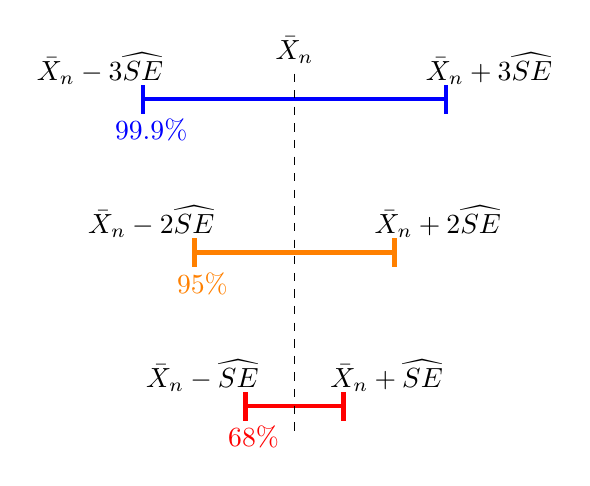
\begin{tikzpicture}[scale = 0.65]
	\draw [ultra thick, blue, |-|](-3,3) -- (3,3);
	\node [above] at (-3.8,3.1) {$\bar{X}_n-3 \widehat{SE}$};
	\node [above] at (3.8,3.1) {$\bar{X}_n+3  \widehat{SE}$};
	\node [below, blue] at (-2.8, 2.8) {99.9\%};	
	
	\draw [ultra thick, orange, |-|](-2,0) -- (2,0);
	\node [above] at (-2.8,0.1) {$\bar{X}_n-2 \widehat{SE}$};
	\node [above] at (2.8,0.1) {$\bar{X}_n+2 \widehat{SE}$};
	\node [below, orange] at (-1.8, -0.2) {95\%};	

	\draw [ultra thick, red, |-|](-1,-3) -- (1,-3);
	\node [above] at (-1.8,-2.9) {$\bar{X}_n -  \widehat{SE}$};
	\node [above] at (1.8,-2.9) {$\bar{X}_n +  \widehat{SE}$};
	\node [below, red] at (-0.8, -3.2) {68\%};	
	
	\draw [dashed](0,3.5) -- (0,-3.5);
	\node [above] at (0,3.5) {$\bar{X}_n$};	
\end{tikzpicture}
\singlespacing
\caption{\small  Each CI gives a range of ``plausible'' values for the population mean $\mu$, centered at the sample mean $\bar{X}_n$. Values near the middle are ``more plausible'' in the sense that a small reduction in confidence level gives a much shorter interval centered in the same place. This is because the sample mean is unlikely to take on values far from the population mean in repeated sampling (CLT).}
\end{figure}

\end{frame}
%%%%%%%%%%%%%%%%%%%%%%%%%%%%%%%%%%%%%%%%
\begin{frame}
\frametitle{CI for Difference of Population Means Using CLT}

\begin{block}{Earlier}
Used CLT to get CI for difference of population proportions based on independent samples.
\end{block}

\begin{block}{But Proportions are a Kind of Mean!}
Population proportion is mean of Bernoulli random variable, and sample proportion is mean of sample comprised of ones and zeros.
\end{block}

\vspace{2em}

\alert{The general problem of constructing a CI for the difference of population means using the CLT is essentially identical to what we did earlier for population proportions.}

\end{frame}

%%%%%%%%%%%%%%%%%%%%%%%%%%%%%%%%%%%%%%%%
\begin{frame}
\frametitle{CI for Difference of Population Means Using CLT}
\begin{block}{Setup: Independent Random Samples}
$X_1, \hdots, X_n \sim \mbox{iid}$ with mean $\mu_X$ and variance $\sigma_X^2$\\ $Y_1, \hdots, Y_m \sim \mbox{iid}$ with mean $\mu_Y$ and variance $\sigma_Y^2$\\
\emph{where each sample is independent of the other } 
\end{block}

\begin{alertblock}{We Do Not Assume the Populations are Normal!}
\end{alertblock}

\end{frame}



%%%%%%%%%%%%%%%%%%%%%%%%%%%%%%%%%%%%%%%%
\begin{frame}
\frametitle{Difference of Sample Means $\bar{X}_n-\bar{Y}_m$ and the CLT}
\begin{block}{What We Have}
Approx.\ sampling dist.\ for \emph{individual}  sample means from CLT:
\alert{$\bar{X}_n\approx N\left(\mu_X, \widehat{SE}(\bar{X}_n)^2\right), \quad \bar{Y}_m\approx N\left(\mu_Y, \widehat{SE}(\bar{Y}_m)^2\right)$}
\end{block}

\begin{block}{What We Want}
Sampling Distribution of the \emph{difference} $\bar{X}_n - \bar{Y}_m$
\end{block}

\begin{block}{Use Independence of the Two Samples}
\alert{$\bar{X}_n - \bar{Y}_m\approx N\left( \mu_X - \mu_Y, \widehat{SE}(\bar{X}_n)^2 +\widehat{SE}(\bar{Y}_m)^2\right)$}



$$\implies \widehat{SE}(\bar{X}_n - \bar{Y}_m) =  \sqrt{\widehat{SE}(\bar{X}_n)^2 +\widehat{SE}(\bar{Y}_m)^2}  = \sqrt{\displaystyle\frac{S_x^2}{n} + \frac{S_y^2}{m} }$$
\end{block}

\end{frame}
%%%%%%%%%%%%%%%%%%%%%%%%%%%%%%%%%%%%%%%%
\begin{frame}
\frametitle{CI for Difference of Pop.\ Means (Independent Samples)}

$X_1, \hdots, X_n \sim \mbox{iid}$ with mean $\mu_X$ and variance $\sigma_X^2$\\ $Y_1, \hdots, Y_m \sim \mbox{iid}$ with mean $\mu_Y$ and variance $\sigma_Y^2$\\
\emph{where each sample is independent of the other } 


	$$\left(\bar{X}_n - \bar{Y}_m\right) \pm \texttt{qnorm}(1-\alpha/2) \sqrt{\frac{S_x^2}{n} + \frac{S_y^2}{m}}$$
	\alert{Approximation based on the CLT. Works well provided $n,m$ large.}
\end{frame}

%%%%%%%%%%%%%%%%%%%%%%%%%%%%%%%%%%%%%%%%
\begin{frame}
\frametitle{Which is the Harder Exam?}
A previous semester's class had two midterms. Here are the scores:
%
\begin{table}[!tbp]
\begin{center}
\begin{tabular}{rrrr}
\hline\hline
\multicolumn{1}{r}{Student}&\multicolumn{1}{r}{Exam 1}&\multicolumn{1}{r}{Exam 2}&\multicolumn{1}{r}{Difference}\tabularnewline
\hline
$ 1$&$57.1$&$60.7$&$  3.6$\tabularnewline
$ 2$&$77.1$&$77.9$&$  0.7$\tabularnewline
$ 3$&$83.6$&$93.6$&$ 10.0$\tabularnewline
\vdots&\vdots&\vdots&\vdots\\
$69$&$75.0$&$74.3$&$ -0.7$\tabularnewline
$70$&$96.4$&$86.4$&$-10.0$\tabularnewline
$71$&$78.6$&$82.9$&$  4.3$\tabularnewline
\hline
Sample Mean: & 79.6 & 81.4  &1.8\\
\hline
\end{tabular}
\end{center}
\end{table}

\alert{Was the second exam easier than the first?}
\end{frame}
%%%%%%%%%%%%%%%%%%%%%%%%%%%%%%%%%%%%%%%%
\begin{frame}
\frametitle{What is the population model?}

\begin{block}{What does it mean to say that one exam is easier?} 
	\begin{itemize}
	\item Exam partly measures what you know and is partly random 
		\begin{itemize}
			\item You could have a bad day
			\item The exam might focus on your weaker areas
		\end{itemize}
	\item If a very large number of students take the exams, the randomness should \emph{average out}.
		\item If a small number of students take the exams, they might score lower on the ``easier exam'' because of bad luck.
	\end{itemize}
\end{block}




 \end{frame}


%%%%%%%%%%%%%%%%%%%%%%%%%%%%%%%%%%%%%%%%
\begin{frame}
\frametitle{Are the two samples independent? }
Suppose we treat the scores on the first midterm as one sample and the scores on the second as another. Are these samples independent?

\begin{enumerate}[(a)]
	\item Yes
	\item No
	\item Not Sure
\end{enumerate}

\pause
\alert{No -- Each sample contains exactly the same students!}

\end{frame}
%%%%%%%%%%%%%%%%%%%%%%%%%%%%%%%%%%%%%%%%
\begin{frame}
\frametitle{Dependent Samples -- Same Students Took Each Exam}
% latex.default(round(grades.out, 1), file = "grades.tex", rowname = NULL) 
%
\begin{table}[!tbp]
\begin{center}
\begin{tabular}{rccr}
\hline\hline
\multicolumn{1}{r}{Student}&\multicolumn{1}{c}{Exam 1}&\multicolumn{1}{c}{Exam 2}&\multicolumn{1}{r}{Difference}\tabularnewline
\hline
$ 1$&$57.1$&$60.7$&$  3.6$\tabularnewline
\vdots&\vdots&\vdots&\vdots\\
$71$&$78.6$&$82.9$&$  4.3$\tabularnewline
\hline
Sample Mean: & 79.6 & 81.4  &1.8\\
%Sample Var. &117  & 151 & 124\\
\alert{Sample Corr.} & \multicolumn{2}{c}{\alert{0.54}}&\\
\hline
\end{tabular}
\caption{The samples are dependent because each includes \emph{exactly the same students}. Indeed, we see that scores on the two exams are strongly positively correlated: students who did well on the first exam tended to do well on the second.}
\end{center}
\end{table}

\end{frame}
%%%%%%%%%%%%%%%%%%%%%%%%%%%%%%%%%%%%%%%%
\begin{frame}
\frametitle{What's going on here?}

We don't really have two samples: we have a \emph{single} sample of students, each of whom took two exams. This is really a \emph{one sample problem} based on the \emph{difference of individual exam scores}. Such a setup is sometimes referred to as \alert{matched pairs data}

\vspace{2em}

\fbox{Let $D_i = X_i - Y_i$ be the difference of student $i$'s exam scores.}

\end{frame}
%%%%%%%%%%%%%%%%%%%%%%%%%%%%%%%%%%%%%%%%
\begin{frame}
\frametitle{Solving this as a One-Sample Problem}
\small
\fbox{Let $D_i = X_i - Y_i$ be the difference of student $i$'s exam scores.}

\vspace{2em}
I calculated the following in R:
	\begin{eqnarray*}
	\bar{D}_n &=& \frac{1}{n}\sum_{i=1}^n D_i \approx 1 .8\\
	S^2_D &=& \frac{1}{n-1}\sum_{i=1}^n (D_i - \bar{D})^2 \approx 	124\\ 
	\widehat{SE}(\bar{D}_n) &=&(S_D /\sqrt{n}) \approx \sqrt{124/71} \approx 1.3 
	\end{eqnarray*}
	
\vspace{1em}
\alert{Approximate 95\% CI Based on the CLT:}
$$\alert{\boxed{1.8 \pm 2.6 = (-0.8, 4.4)}} \quad \mbox{What is our conclusion?}$$

\end{frame}
%%%%%%%%%%%%%%%%%%%%%%%%%%%%%%%%%%%%%%%%
\begin{frame}
	\begin{center}
	\Huge How are the Independent Samples and Matched Pairs Problems Related?
	\end{center}
\end{frame}

%%%%%%%%%%%%%%%%%%%%%%%%%%%%%%%%%%%%%%%%
\begin{frame}
\frametitle{Difference of Means = Mean of Differences?}
\fbox{Let $D_i = X_i - Y_i$ be the difference of student $i$'s exam scores.}

True or False:
	$$\bar{D}_n = \bar{X}_n - \bar{Y}_n$$

\begin{enumerate}[(a)]
	\item True
	\item False
	\item Not Sure
\end{enumerate}

\end{frame}
%%%%%%%%%%%%%%%%%%%%%%%%%%%%%%%%%%%%%%%%
\begin{frame}
\frametitle{Difference of Means Equals Mean of Differences}
\fbox{Let $D_i = X_i - Y_i$ be the difference of student $i$'s exam scores.}

\vspace{1em}
\alert{Sample mean of differences \emph{equals} difference of sample means}
\begin{eqnarray*}
	\bar{D}_n &=& \frac{1}{n}\sum_{i=1}^n D_i = \frac{1}{n}\sum_{i=1}^n (X_i - Y_i)\\
	& =& \left(\frac{1}{n}\sum_{i=1}^n X_i \right)- \left(\frac{1}{n}\sum_{i=1}^n Y_i \right)= \bar{X}_n - \bar{Y}_n
\end{eqnarray*}



\vspace{2em}

\alert{Linearity of Expectation holds even under dependence:}
\begin{eqnarray*}
	E[\bar{D}_n] = E[\bar{X}_n - \bar{Y}_n] = E[\bar{X}_n] - E[\bar{Y}_n] = \mu_X - \mu_Y
\end{eqnarray*}


\end{frame}

%%%%%%%%%%%%%%%%%%%%%%%%%%%%%%%%%%%%%%%%
\begin{frame}
\frametitle{Exam Dataset}
% latex.default(round(grades.out, 1), file = "grades.tex", rowname = NULL) 
%
\begin{table}[!tbp]
\begin{center}
\begin{tabular}{rccr}
\hline\hline
\multicolumn{1}{r}{Student}&\multicolumn{1}{c}{Exam 1}&\multicolumn{1}{c}{Exam 2}&\multicolumn{1}{r}{Difference}\tabularnewline
\hline
$ 1$&$57.1$&$60.7$&$  3.6$\tabularnewline
\vdots&\vdots&\vdots&\vdots\\
$71$&$78.6$&$82.9$&$  4.3$\tabularnewline
\hline
Sample Mean: & 79.6 & 81.4  &1.8\\
\hline
\end{tabular}
\end{center}
\end{table}


\begin{eqnarray*}
	\bar{D}_n &=& 1.8\\ 
	\bar{X}_n - \bar{Y}_n &=&  81.4 - 79.6 =   1.8  \;\alert{\checkmark}
\end{eqnarray*}

\end{frame}

%%%%%%%%%%%%%%%%%%%%%%%%%%%%%%%%%%%%%%%%

\begin{frame}
\frametitle{...But Dependence Changes the Variance Calculation}
\small
Recall that for any two RVs $X,Y$ and constants $a,b$
$$Var(aX + bY) = a^2 Var(X) + b^2Var(Y) + 2ab Cov(X,Y)$$

\pause
From the last slide, $\bar{D}_n = \bar{X}_n - \bar{Y}_n$, hence
\begin{eqnarray*}
Var(\bar{D}_n) &=& Var(\bar{X}_n - \bar{Y}_n)\\ \pause
 &=& Var(\bar{X}_n) + Var(\bar{Y}_n) - 2Cov(\bar{X}_n, \bar{Y}_n)\\ \pause
	&=& \frac{\sigma_X^2}{n} + \frac{\sigma_Y^2}{n} - 2Cov(\bar{X}_n, \bar{Y}_n) \alert{\neq \frac{\sigma_X^2}{n} + \frac{\sigma_Y^2}{n}}\\
\end{eqnarray*}


\alert{Since the samples are correlated, $Cov(\bar{X}_n, \bar{Y}_n)\neq 0$! Hence the standard error estimate for independent samples, $\sqrt{S^2_X/n + S^2_Y/n}$, is  inappropriate!}


\end{frame}
%%%%%%%%%%%%%%%%%%%%%%%%%%%%%%%%%%%%%%%%

\begin{frame}
\frametitle{Another Way to Calculate Sample Var.\ of the Differences}
\footnotesize
Variance of the differences can also be calculated from the sample variance for each exam along with the correlation between them:
\begin{eqnarray*}
	S_D^2&=& \frac{1}{n-1}\sum_{i=1}^n \left( D_i - \bar{D}_n\right)^2 = \pause \frac{1}{n-1}\sum_{i=1}^n \left[ \left( X_i - Y_i\right) - \left( \bar{X}_n - \bar{Y}_n\right)\right]^2\\ \pause
	&=&\frac{1}{n-1}\sum_{i=1}^n \left[ \left( X_i - \bar{X}_n\right) - \left( Y_i - \bar{Y}_n\right)\right]^2\\ \pause
	&=&\frac{1}{n-1}\sum_{i=1}^n \left[ \left( X_i - \bar{X}_n\right)^2 + \left( Y_i - \bar{Y}_n\right)^2 - 2\left(X_i - \bar{X}_n\right)\left(Y_i - \bar{Y}_n\right)\right]\\ \pause
	&=& S_X^2 + S_Y^2 - 2 S_{XY}\\ \pause
	&=& S_X^2 + S_Y^2 - 2 S_X S_Y r_{XY}
\end{eqnarray*}

\vspace{1em}
\alert{$\boxed{r_{XY} > 0 \implies S_D^2 < S_X^2 + S_Y^2}$}

\end{frame}
%%%%%%%%%%%%%%%%%%%%%%%%%%%%%%%%%%%%%%%%
\begin{frame}
\frametitle{Dependent Samples -- Calculating the ME}
% latex.default(round(grades.out, 1), file = "grades.tex", rowname = NULL) 
%
\begin{table}[!tbp]
\begin{center}
\begin{tabular}{rccr}
\hline\hline
\multicolumn{1}{r}{Student}&\multicolumn{1}{c}{Exam 1}&\multicolumn{1}{c}{Exam 2}&\multicolumn{1}{r}{Difference}\tabularnewline
\hline
$ 1$&$57.1$&$60.7$&$  3.6$\tabularnewline
\vdots&\vdots&\vdots&\vdots\\
$71$&$78.6$&$82.9$&$  4.3$\tabularnewline
\hline
Sample Var. &117  & 151 & \alert{\fbox{?}}\\
Sample Corr.& \multicolumn{2}{c}{0.54}&\\
\hline
\end{tabular}
\end{center}
\end{table}

$$117 + 151 - 2 \times 0.54 \times \sqrt{117 \times 151} \approx 124   \;\alert{\checkmark}$$

\alert{This agrees with what we got when we did calculations directly for the differences!}
\end{frame}
%%%%%%%%%%%%%%%%%%%%%%%%%%%%%%%%%%%%%%%%
\begin{frame}
\frametitle{The ``Wrong CI'' (Assuming Independence) is Too Wide}
\footnotesize
% latex.default(round(grades.out, 1), file = "grades.tex", rowname = NULL) 
%
\begin{table}[!tbp]
\begin{center}
\begin{tabular}{rccr}
\hline\hline
\multicolumn{1}{r}{Student}&\multicolumn{1}{c}{Exam 1}&\multicolumn{1}{c}{Exam 2}&\multicolumn{1}{r}{Difference}\tabularnewline
\hline
Sample Size & 71 & 71 & 71\\
Sample Mean & 79.6 & 81.4  &1.8\\
Sample Var. &117  & 151 & 124\\
Sample Corr.& \multicolumn{2}{c}{0.54}&\\
\hline
\end{tabular}
\end{center}
\end{table}

\singlespacing
\small

\begin{block}{Wrong Interval -- Assumes Independence}
$$1.8 \pm 2\times  \sqrt{117/71 + 151/71} \implies (-2.1, 5.7)$$
\end{block}

\pause

\begin{block}{Correct Interval -- Matched Pairs}
$$1.8 \pm 2\times  \sqrt{124/71} \implies (-0.8, 4.4)$$
\end{block}

\pause
\alert{Top CI is too wide because the exam scores are positively correlated, so the variance of the differences is less than the sum of the variances of the two exams. Both CIs, however, are correctly centered.}

\end{frame}
%%%%%%%%%%%%%%%%%%%%%%%%%%%%%%%%%%%%%%%%


\begin{frame}
\frametitle{Overview: Independent Samples Versus Matched Pairs}

\begin{itemize}
	\item When you see a problem that involves two datasets, think carefully about whether they should be treated as independent samples or if they're really matched pairs. The CIs differ! 
	\item The matched pairs calculations can be done in two ways: 
		\begin{enumerate}
			\item Direct calculation using the sample mean and standard deviation of the individual differences $D_i = X_i - Y_i$ 
			\item Indirect calculation using the sample mean and standard deviation of the X's and Y's \emph{separately} along with the sample correlation between them. 
		\end{enumerate}
\end{itemize}
\end{frame}


%%%%%%%%%%%%%%%%%%%%%%%%%%%%%%%%%%%%%%%%
\begin{frame}
\begin{center}
	\huge Refined 95\% CI for Proportion: \\``Add Two Successes and Failures''
\end{center}
\end{frame}
%%%%%%%%%%%%%%%%%%%%%%%%%%%%%%%%%%%%%%%%
\begin{frame}
\frametitle{Refined 95\% CI for Population Proportion}
\small
\alert{\fbox{Add four ``fake'' observations to the dataset: two zeros and two ones.}}
\vspace{1em}

\begin{columns}

\column{0.5\textwidth}
\begin{block}{Textbook Confidence Interval}
$$\widehat{p} = \frac{1}{n}\left(\sum_{i=1}^n X_i\right)$$

$$\widehat{p}\pm \texttt{qnorm}\left(0.975\right) \times\sqrt{\frac{\widehat{p}(1-\widehat{p})}{n}}$$
\end{block}

\column{0.5\textwidth}
\begin{block}{Refined Confidence Interval}
$$\alert{\widetilde{p}} = \frac{1}{n+\alert{4}} \left(\alert{2}+ \sum_{i=1}^n X_i\right)$$

$$\alert{\widetilde{p}} \pm \texttt{qnorm}\left(0.975\right) \times \sqrt{\frac{\alert{\widetilde{p}}(1-\alert{\widetilde{p}})}{n+\alert{4}}}$$

\end{block}

\end{columns}

\vspace{1em}

\alert{This is related to problem 7-13 in the textbook...}
\end{frame}
%%%%%%%%%%%%%%%%%%%%%%%%%%%%%%%%%%%%%%%%
\begin{frame}
\frametitle{Refined 95\% CI for Difference of Population Proportions}
\small
\alert{\fbox{Add four ``fake'' observations total: two to \emph{each} dataset (a one and a zero).}}

\begin{block}{Textbook Confidence Interval}
$$\widehat{p} - \widehat{q} = \frac{1}{n}\left(\sum_{i=1}^n X_i\right) - \frac{1}{m}\left(\sum_{i=1}^n Y_i\right)$$

	$$\left(\widehat{p} -\widehat{q}\right)\pm \texttt{qnorm}(0.975) \times \sqrt{\frac{\widehat{p}(1-\widehat{p})}{n} + \frac{\widehat{q}(1-\widehat{q})}{m}}$$

\end{block}


\begin{block}{Refined Confidence Interval}
	$$\alert{p^*} - \alert{q^*} = \frac{1}{n+\alert{2}}\left(1 + \sum_{i=1}^n X_i\right) - \frac{1}{m+\alert{2}}\left(1 + \sum_{i=1}^m Y_i\right) $$

	$$\left(\alert{p^*} -\alert{q^*}\right)\pm \texttt{qnorm}(0.975) \times \sqrt{\frac{\alert{p^*}(1-\alert{p^*})}{n+\alert{2}} + \frac{\alert{q^*}(1-\alert{q^*})}{m+\alert{2}}}$$
\end{block}

\end{frame}
%%%%%%%%%%%%%%%%%%%%%%%%%%%%%%%%%%%%%%%%
\begin{frame}
\frametitle{What is the point of this?}

\begin{block}{Recall from Last Time}
Our CIs for proportions are \emph{approximations} based on the CLT. 
\end{block}

\begin{block}{When is the approximation good?} 
Large sample size (n,m) and true population proportions (p,q) that aren't too close to zero or one. 
\end{block}


\begin{alertblock}{Why the Refined Intervals?}
They work well even when sample sizes ($n,m$) are small and true population proportions ($p,q$) are close to zero or one. When the samples are large, the refined intervals are practically identical to the textbook intervals. 
\end{alertblock}
\end{frame}
%%%%%%%%%%%%%%%%%%%%%%%%%%%%%%%%%%%%%%%%
\begin{frame}
	\frametitle{Confidence Intervals We've Covered}
	\begin{enumerate}
		\item Exact CIs based on assumption of Normality:
			\begin{enumerate}[(a)]
				\item CI for population mean, population variance known (\texttt{qnorm})
				\item CI for population mean, population variance unknown (\texttt{qt})
				\item CI for population variance (\texttt{qhisq})
				\item CI for difference of population means, indep.\ samples (\texttt{qt})
			\end{enumerate}
		\item Approximate CIs using CLT (\texttt{qnorm})
			\begin{enumerate}[(a)]
				\item CI for population mean (also matched pairs data)
				\item CI for difference of population means, independent samples
				\item CIs for proportions and differences of proportions 
					\begin{enumerate}[(i)]
						\item ``Textbook'' version -- use sample proportions
						\item ``Refined'' version -- ``add two successes and failures (total)''			
					\end{enumerate}
			\end{enumerate}
	\end{enumerate}
  \alert{In nearly all real applications we'll use 2, but you need to understand what's going on in 1 as well.}
\end{frame}
%%%%%%%%%%%%%%%%%%%%%%%%%%%%%%%%%%%%%%%%

\end{document}